% =============================================================
% BAO CAO HOC PHAN - HE HO TRO QUYET DINH
% De tai: Pizza Delivery DSS
% Bien dich: xelatex main.tex (hai lan)
% =============================================================
\documentclass[12pt,a4paper,oneside]{report}

\usepackage{fontspec}
\setmainfont{Times New Roman}
\IfFontExistsTF{Cascadia Mono}
  {\newfontfamily\monofont{Cascadia Mono}}
  {\newfontfamily\monofont{Courier New}}

\usepackage[a4paper,margin=2.5cm,headheight=16pt]{geometry}
\usepackage{indentfirst}
\usepackage{setspace}
\onehalfspacing
\setlength{\parindent}{0.5cm}
\setlength{\parskip}{2pt}

\usepackage[table,dvipsnames]{xcolor}
\definecolor{HUSTBlue}{RGB}{0,51,102}
\definecolor{HUSTRed}{RGB}{197,24,24}
\definecolor{boxgray}{RGB}{247,247,247}
\definecolor{linkcol}{RGB}{0,71,133}

\usepackage{amsmath,amssymb,bm}
\usepackage{graphicx}
\graphicspath{{../figures/}{assets/}}
\usepackage{float}
\usepackage{caption}
\usepackage{subcaption}
\captionsetup{
  font=small,
  labelfont={bf,color=HUSTBlue},
  justification=centering,
  skip=6pt
}
\usepackage{booktabs,array,multirow,longtable,tabularx}
\usepackage{enumitem}
\renewcommand{\arraystretch}{1.18}

\usepackage[most]{tcolorbox}
\newtcolorbox{insight}[1][]{
  enhanced,breakable,boxrule=0.6pt,colback=boxgray,colframe=HUSTBlue,
  arc=2pt,left=8pt,right=8pt,top=6pt,bottom=6pt,fonttitle=\bfseries,
  title={#1}
}

\usepackage{tikz}
\usetikzlibrary{arrows.meta,positioning,shapes.geometric,calc}

\usepackage{fancyhdr}
\pagestyle{fancy}
\fancyhf{}
\fancyhead[L]{\small\itshape\nouppercase{\leftmark}}
\fancyhead[R]{\small\thepage}
\renewcommand{\headrulewidth}{0.4pt}
\fancypagestyle{plain}{
  \fancyhf{}
  \fancyfoot[C]{\small\thepage}
  \renewcommand{\headrulewidth}{0pt}
}

\usepackage{titlesec}
\titleformat{\chapter}[hang]
  {\LARGE\bfseries\color{HUSTBlue}}
  {\colorbox{HUSTBlue}{\color{white}\rule[-6pt]{0pt}{28pt}\,\thechapter\,}}
  {14pt}{\LARGE}
\titlespacing*{\chapter}{0pt}{10pt}{24pt}
\titleformat{\section}
  {\Large\bfseries\color{HUSTBlue}}{\thesection}{0.8em}{}
\titleformat{\subsection}
  {\large\bfseries\color{HUSTBlue}}{\thesubsection}{0.8em}{}

\renewcommand{\chaptername}{Chương}
\renewcommand{\contentsname}{Mục lục}
\renewcommand{\figurename}{Hình}
\renewcommand{\tablename}{Bảng}
\renewcommand{\listfigurename}{Danh sách hình}
\renewcommand{\bibname}{Tài liệu tham khảo}
\renewcommand{\appendixname}{Phụ lục}

\usepackage[unicode]{hyperref}
\hypersetup{
  colorlinks=true,
  linkcolor=linkcol,
  citecolor=HUSTRed,
  urlcolor=linkcol,
  pdftitle={He ho tro quyet dinh dieu phoi giao pizza},
  pdfauthor={Nhom 29}
}

\newcommand{\code}[1]{\nolinkurl{#1}}

\begin{document}
\pagenumbering{roman}

\begin{titlepage}
\centering
\begin{tikzpicture}[remember picture,overlay]
  \draw[HUSTBlue,line width=1pt,dash pattern=on 6pt off 3pt]
    ($(current page.north west)+(1.4cm,-1.4cm)$) rectangle
    ($(current page.south east)+(-1.4cm,1.4cm)$);
  \draw[HUSTBlue,line width=0.4pt]
    ($(current page.north west)+(1.65cm,-1.65cm)$) rectangle
    ($(current page.south east)+(-1.65cm,1.65cm)$);
\end{tikzpicture}

{\large\bfseries ĐẠI HỌC BÁCH KHOA HÀ NỘI\par}
{\large\bfseries KHOA TOÁN -- TIN\par}
\vspace{2pt}{\color{HUSTBlue}\rule{3cm}{0.8pt}}\par
\vspace{0.8cm}

\begin{tabular}{c@{\hskip 1.6cm}c}
  
\includegraphics[height=2.6cm]{logo_bachkhoa.png}
  &
  
\includegraphics[height=2.6cm]{logo_toantin.png}
\end{tabular}

\vspace{1cm}
{\Large\bfseries BÁO CÁO BÀI TẬP NHÓM\par}
\vspace{4pt}
{\large HỌC PHẦN HỆ HỖ TRỢ QUYẾT ĐỊNH\par}
\vspace{0.9cm}
{\color{HUSTBlue}\LARGE\bfseries
HỆ HỖ TRỢ QUYẾT ĐỊNH ĐIỀU PHỐI GIAO PIZZA\par}
\vspace{5pt}
{\color{HUSTBlue}\LARGE\bfseries
DỰA TRÊN DỰ BÁO ĐƠN GIAO TRỄ\par}
\vspace{6pt}
{\large\itshape
A Decision Support System for Pizza Delivery Operations\par}
\vspace{1.2cm}

{\large
\begin{tabular}{r@{\hskip 0.6cm}l}
  \textbf{Giảng viên:} & TS. Lê Hải Hà\\[4pt]
  \textbf{Giảng viên giao đề tài:} & TS. Trịnh Đình Thăng\\[4pt]
  \textbf{Nhóm thực hiện:} & Nhóm 29\\[4pt]
  \textbf{Học kỳ:} & 2025--2026\\
\end{tabular}\par}

\vfill
{\bfseries Hà Nội, tháng 6 năm 2026\par}
\end{titlepage}

\clearpage
\chapter*{Bảng phân công công việc}
\addcontentsline{toc}{chapter}{Bảng phân công công việc}

\begin{table}[H]
\centering
\small
\caption*{Phân công và tỷ lệ đóng góp của các thành viên Nhóm 29}
\begin{tabularx}{\textwidth}{p{2.7cm}p{1.6cm}X p{0.9cm}p{3.1cm}}
\toprule
\textbf{Thành viên} & \textbf{MSSV} & \textbf{Công việc chính} &
\textbf{Tỷ lệ} & \textbf{Minh chứng}\\
\midrule
Đoàn Danh Long & 20237354 & Điều phối pipeline DSS, mô hình hóa và tổng hợp báo cáo & 25\% & \code{modeling.py}, NB03, \code{model\_summary.json}, báo cáo\\
Vũ Quang Vinh & 20237408 & EDA, customer behavior và kiểm định giả thiết & 25\% & \code{eda.py}, NB02, \code{hypothesis\_tests.csv}\\
Nguyễn Đăng Đức & 20237312 & Feature engineering, forecasting, recommendation và Power BI pack & 25\% & \code{business\_analysis.py}, NB05, \code{powerbi/}\\
Nguyễn Tuấn Anh & 20237293 & Dashboard Streamlit, tối ưu vận tải, kiểm thử & 25\% & \code{streamlit\_app.py}, \code{transport\_optimization.py}, \code{tests/}\\
\bottomrule
\end{tabularx}
\end{table}

\chapter*{Lời mở đầu}
\addcontentsline{toc}{chapter}{Lời mở đầu}

Trong vận hành giao đồ ăn, một đơn giao trễ không chỉ là một lỗi thời gian mà
còn tác động đến trải nghiệm khách hàng, chi phí chăm sóc khách hàng và khối
lượng điều phối. Nếu chỉ nhìn từng đơn riêng lẻ, người quản lý khó biết đơn nào
nên được theo dõi trước, ca nào cần tài xế dự phòng và thời điểm nào cần bố trí
thêm nhân sự. Một hệ hỗ trợ quyết định vì vậy cần kết hợp dữ liệu, mô hình dự
báo và quy tắc vận hành minh bạch để đưa ra khuyến nghị có thể kiểm tra.

Báo cáo này trình bày một nguyên mẫu DSS trên bộ dữ liệu pizza delivery của
Kaggle. Do dữ liệu có nhiều dấu hiệu được sinh tự động, nhóm không xem bộ dữ
liệu như log vận hành thật hoàn chỉnh. Ngược lại, điểm yếu này được đưa vào
quy trình học thuật: audit leakage, reverse-engineering generator, đánh giá mô
hình trên train/dev/test, sau đó chuyển kết quả dự báo thành hàng đợi ưu tiên,
dashboard và kịch bản tối ưu phân công tài xế.

\chapter*{Tóm tắt}
\addcontentsline{toc}{chapter}{Tóm tắt}

Báo cáo xây dựng một Hệ hỗ trợ quyết định điều phối giao pizza dựa trên dữ liệu
1.004 đơn hàng từ Kaggle. Mục tiêu là dự báo khả năng đơn hàng bị giao trễ trước
khi đơn hoàn tất, đồng thời hỗ trợ phân tích hành vi khách hàng, dự báo nhu cầu
minh họa, đề xuất staffing và tạo hàng đợi ưu tiên cho điều phối.

Quy trình gồm bảy phần: xác định bài toán DSS; audit dữ liệu và chống leakage;
phân tích dữ liệu synthetic; EDA và kiểm định giả thiết; xây dựng mô hình dự
báo; chuyển dự báo thành Risk Score, Priority và Recommended Action; cuối cùng
là dashboard Streamlit, Power BI data pack và kịch bản assignment theo tinh
thần bài toán vận tải. Vì nguồn dữ liệu chỉ cung cấp nhãn
\code{is\_delayed} mà không mô tả SLA, nhóm suy luận ranh giới nhãn bằng cách
thử các luật ngưỡng trên \code{delivery\_duration\_min}. Kết quả cho thấy các
đơn đúng giờ có duration lớn nhất 30 phút, các đơn trễ có duration nhỏ nhất
35 phút; do duration nằm trên lưới 5 phút, hai luật \code{duration > 30} và
\code{duration >= 35} là tương đương trên dataset. Mô hình Logistic Regression
trên feature set compact được chọn theo F2 trên dev và đạt trên test: Accuracy
0,9602; Balanced Accuracy 0,9661; F1 0,9111; F2 0,9491; MCC 0,8889. Tuy vậy,
vì dữ liệu có tính synthetic, các phân tích forecast, preference và brand được
diễn giải như minh họa phương pháp, không phải kết luận kinh doanh sản xuất.

\vspace{6pt}
\noindent\textbf{Từ khóa:} DSS, Pizza Delivery, Supervised Learning, Data
Forensics, Forecasting, Transportation Assignment, Dashboard.

\chapter*{Tám câu hỏi bắt buộc}
\addcontentsline{toc}{chapter}{Tám câu hỏi bắt buộc}

Theo hướng dẫn học phần, báo cáo trả lời trực diện tám câu hỏi sau; chi tiết nằm
ở các chương được dẫn chiếu.

\begin{longtable}{>{\bfseries}p{5.3cm}p{9.0cm}}
\toprule
\textmd{\bfseries Câu hỏi} & \textbf{Trả lời ngắn (chi tiết ở chương)}\\
\midrule
\endhead
Bài toán thực tế là gì? & Dự báo đơn pizza có nguy cơ giao trễ \emph{trước khi
giao} để hỗ trợ điều phối (Chương 1).\\
Ai dùng kết quả? & Quản lý vận hành / điều phối viên của chuỗi giao pizza
(Chương 1).\\
Người dùng cần ra quyết định gì? & Đơn nào theo dõi/ưu tiên trước, khi nào chuẩn
bị tài xế dự phòng, gửi cảnh báo khách (Chương 1, 6).\\
Dữ liệu nào được dùng? & 1.004 đơn Kaggle (37 cột sau FE); chỉ dùng feature
biết trước khi giao, cấm cột leakage (Chương 3).\\
Xử lý \& phân tích thế nào? & Audit + chống leakage + split stratified; EDA,
kiểm định, forensics; so sánh 6 model + CV, chọn theo F2 (Chương 3--5).\\
Kết quả quan trọng nhất? & Logistic Regression compact: test F2 0,9491; MCC
0,8889 (kèm CI bootstrap); vượt cả hai baseline (Chương 5).\\
Đề xuất hành động nào? & Risk Score $\to$ Priority $\to$ Recommended Action +
hàng đợi + gán tài xế; xem mục Khuyến nghị (Chương 6).\\
Hạn chế/rủi ro/điều kiện áp dụng? & Dữ liệu synthetic gần tất định, n nhỏ; điểm
cao không phản ánh năng lực dự báo thật; forecast/brand chỉ minh họa
(Chương 6--7).\\
\bottomrule
\end{longtable}

\chapter*{Bảng thuật ngữ}
\addcontentsline{toc}{chapter}{Bảng thuật ngữ}

\begin{longtable}{>{\bfseries}p{4.0cm}p{10.2cm}}
\toprule
\textmd{\bfseries Thuật ngữ} & \textbf{Giải nghĩa}\\
\midrule
\endhead
DSS & Decision Support System -- Hệ hỗ trợ quyết định; hệ thống kết hợp dữ
liệu, mô hình và giao diện để hỗ trợ con người ra quyết định.\\
Đơn trễ & Đơn có \code{is\_delayed = True}; trong dataset này nhãn có ranh
giới quan sát giữa 30 và 35 phút giao hàng.\\
Leakage & Rò rỉ thông tin tương lai vào feature, làm metric mô hình bị ảo.\\
Feature compact & Tập feature đã loại các cột công thức/trùng thông tin, chỉ
giữ biến có thể biết tại thời điểm nhận đơn.\\
Dev set & Tập phát triển dùng để chọn mô hình/siêu tham số trước khi báo test.\\
Hyperparameter tuning & Dò siêu tham số bằng train/CV/dev; không dùng test để
chọn cấu hình nhằm tránh leakage.\\
GridSearchCV & Thử toàn bộ lưới siêu tham số bằng cross-validation rồi chọn cấu
hình có metric trung bình tốt nhất.\\
F2 & Chỉ số F-score đặt trọng số Recall cao hơn Precision; phù hợp khi bỏ sót
đơn trễ là lỗi quan trọng.\\
MCC & Matthews Correlation Coefficient; chỉ số cân bằng cho bài toán nhị phân
mất cân bằng.\\
Data forensics & Phân tích truy ngược dấu vết sinh dữ liệu: công thức tất định,
lượng tử hóa, tính đồng đều và tín hiệu artifact.\\
Risk Score & Điểm rủi ro do tầng DSS tính từ xác suất mô hình và các yếu tố
vận hành.\\
Priority & Mức ưu tiên Low/Medium/High suy từ Risk Score để sắp xếp hàng đợi.\\
Assignment & Bài toán gán đơn cho tài xế giả lập theo chi phí nhỏ nhất; trong
dự án chỉ là kịch bản prescriptive demo.\\
\bottomrule
\end{longtable}

\tableofcontents
\listoffigures
\cleardoublepage
\pagenumbering{arabic}

\chapter{Giới thiệu bài toán}

\section{Bối cảnh và động cơ}

Các nền tảng giao đồ ăn vận hành trong môi trường có nhiều biến động: khoảng
cách đơn hàng, traffic, giờ cao điểm, đặc điểm đơn, phương thức thanh toán và
khả năng đáp ứng của nhân sự. Một quyết định vận hành thường không thể chỉ dựa
trên trực giác từng đơn. Người quản lý cần một hệ thống giúp trả lời:

\begin{enumerate}[leftmargin=*]
  \item đơn nào có nguy cơ giao trễ trước khi đơn hoàn tất;
  \item yếu tố nào đang làm tăng rủi ro trễ;
  \item đơn nào cần theo dõi hoặc can thiệp trước;
  \item khung giờ nào cần bố trí thêm nhân sự;
  \item kết quả phân tích nên được trình bày thế nào để ra quyết định.
\end{enumerate}

Dự án đặt bài toán không chỉ là ``dự báo đúng/sai'', mà là xây dựng một DSS có
đủ ba lớp: phân tích dữ liệu, mô hình dự báo và khuyến nghị hành động. Mô hình
học máy chỉ là một thành phần tạo bằng chứng; quyết định cuối cùng vẫn thuộc về
người quản lý.

\section{Phạm vi đề tài}

Dữ liệu sử dụng là bộ \emph{Pizza Delivery Data with Enhanced Features} trên
Kaggle. Dự án không kết nối hệ thống đặt hàng thật, không định vị tài xế thật,
không gửi thông báo cho khách hàng và không tự động điều phối. Đầu ra trong
phạm vi môn học gồm:

\begin{itemize}[leftmargin=*]
  \item bộ dữ liệu đã chuẩn hóa và split train/dev/test;
  \item phân tích EDA, kiểm định giả thiết, data forensics và customer behavior;
  \item mô hình dự báo \code{is\_delayed};
  \item Risk Score, Priority và Recommended Action;
  \item dashboard Streamlit và Power BI-ready data pack;
  \item kịch bản phân công tài xế giả lập theo chi phí.
\end{itemize}

\section{Câu hỏi nghiên cứu và quyết định}

Báo cáo được tổ chức quanh các câu hỏi sau:

\begin{enumerate}[leftmargin=*]
  \item Dataset có đủ tin cậy để dùng như log vận hành thật không?
  \item Có thể phát hiện và loại bỏ leakage trong bài toán dự báo đơn trễ không?
  \item Những biến trước giao hàng nào liên quan đến rủi ro trễ?
  \item Mô hình nào phù hợp nhất khi chọn trên dev và báo test một lần?
  \item Làm thế nào chuyển xác suất trễ thành khuyến nghị vận hành dễ hiểu?
  \item Có thể minh họa forecasting, recommendation và tối ưu vận tải trong
        phạm vi dataset nhỏ này không?
\end{enumerate}

\begin{insight}[Quan điểm xuyên suốt]
Vì dữ liệu có nhiều dấu hiệu synthetic, báo cáo ưu tiên tính trung thực học
thuật: kết quả mô hình và dashboard được trình bày như nguyên mẫu DSS, còn các
kết luận forecast, preference và brand không được diễn giải như bằng chứng thị
trường thật.
\end{insight}

\chapter{Cơ sở lý thuyết và phương pháp luận}

\section{Khái niệm hệ hỗ trợ quyết định}

Hệ hỗ trợ quyết định là hệ thống thông tin kết hợp dữ liệu, mô hình phân tích
và giao diện tương tác để hỗ trợ con người trong các bài toán bán cấu trúc hoặc
khó tự động hóa hoàn toàn \cite{power2002}. Trong dự án này, DSS không thay
người quản lý quyết định, mà cung cấp:

\begin{itemize}[leftmargin=*]
  \item bằng chứng dữ liệu: tỷ lệ trễ, phân bố đơn, kiểm định giả thiết;
  \item bằng chứng dự báo: xác suất đơn bị trễ và metric đánh giá;
  \item chính sách hành động: Risk Score, Priority và khuyến nghị xử lý.
\end{itemize}

Theo chu trình ra quyết định của Simon \cite{simon1960}, dự án bao phủ các pha:
nhận biết vấn đề qua audit/EDA, thiết kế phương án qua model và rule DSS, lựa
chọn qua Priority/Recommended Action, còn pha thực thi ngoài đời được ghi là
hướng phát triển vì dataset không có phản hồi vận hành thật.

\section{Pipeline phân tích dữ liệu}

\begin{figure}[H]
\centering
\begin{tikzpicture}[
  node distance=6mm and 7mm,
  box/.style={draw=HUSTBlue,rounded corners=2pt,fill=boxgray,align=center,
    text width=2.6cm,minimum height=1.05cm},
  arrow/.style={-{Latex[length=2.2mm]},thick,HUSTBlue}
]
\node[box] (data) {Dữ liệu Kaggle};
\node[box,right=of data] (audit) {Audit\\leakage};
\node[box,right=of audit] (eda) {EDA\\forensics};
\node[box,right=of eda] (model) {Mô hình\\dự báo};
\node[box,below=of model] (dss) {Risk\\Priority};
\node[box,left=of dss] (bi) {Dashboard\\Power BI};
\node[box,left=of bi] (assign) {Assignment\\scenario};
\draw[arrow] (data) -- (audit);
\draw[arrow] (audit) -- (eda);
\draw[arrow] (eda) -- (model);
\draw[arrow] (model) -- (dss);
\draw[arrow] (dss) -- (bi);
\draw[arrow] (dss) -- (assign);
\end{tikzpicture}
\caption{Quy trình logic của hệ hỗ trợ quyết định giao pizza.}
\end{figure}

Pipeline được thiết kế theo nguyên tắc: mọi biến dùng để dự báo phải biết trước
hoặc tại thời điểm nhận đơn; mô hình được fit trên train, chọn trên dev và báo
test sau khi khóa.

\section{Các kỹ thuật sử dụng}

\subsection{Phân tích mô tả, kiểm định và data forensics}

EDA trả lời dữ liệu có đặc điểm gì; kiểm định giả thiết đánh giá mối liên hệ
giữa biến categorical và nhãn trễ; data forensics truy ngược dấu vết sinh dữ
liệu. Ba nhóm kỹ thuật này giúp phân biệt insight có ý nghĩa vận hành với
artifact do generator tạo ra.

Các kiểm định trong dự án gồm chi-square independence cho biến categorical,
goodness-of-fit với phân phối đều, mutual information trước/sau khi kiểm soát
distance band và ablation feature trong mô hình.

\subsection{Mô hình phân loại}

Bài toán dự báo \code{is\_delayed} là phân loại nhị phân mất cân bằng. Dự án so
sánh Logistic Regression, Decision Tree, Gaussian Naive Bayes, k-NN, SVM và
Random Forest. Các biến số được chuẩn hóa, biến categorical được one-hot
encoding trong pipeline scikit-learn để tránh fit transform sai split.

Metric chính là F2 vì bỏ sót đơn trễ thường bất lợi hơn cảnh báo dư. Tuy vậy,
F2 được báo cùng Accuracy, Balanced Accuracy, F1 và MCC để tránh diễn giải một
chiều.

\subsection{Forecasting, recommendation và tối ưu vận tải}

Forecasting được dùng để minh họa planning: dự báo tổng đơn theo tháng và share
size/type bằng seasonal-naive. Recommendation dùng luật phổ biến theo context
(nhà hàng, size, location, time segment). Tối ưu vận tải được mô phỏng bằng bài
toán assignment chi phí nhỏ nhất trên nhóm đơn High priority; driver/fleet là
giả lập vì dataset không có bảng tài xế thật.

\chapter{Dữ liệu và kiểm soát chất lượng}

\section{Nguồn dữ liệu}

Dataset được lấy từ Kaggle:

\begin{center}
\code{akshaygaikwad448/pizza-delivery-data-with-enhanced-features}
\end{center}

File gốc là \code{Enhanced\_pizza\_sell\_data\_2024-25.xlsx}. Sau chuẩn hóa tên
cột và feature engineering, dataset có 37 cột.

\begin{table}[H]
\centering
\caption{Tóm tắt dữ liệu}
\begin{tabular}{lr}
\toprule
Chỉ tiêu & Giá trị\\
\midrule
Số đơn hàng & 1.004\\
Số cột gốc & 25\\
Số cột sau feature engineering & 37\\
Missing value & 0\\
Duplicate order id & 0\\
Đơn trễ & 210\\
Đơn đúng giờ & 794\\
Tỷ lệ trễ & 20,92\%\\
Thời gian nhỏ nhất & 2024-01-05\\
Thời gian lớn nhất & 2026-07-07\\
\bottomrule
\end{tabular}
\end{table}

\section{Suy luận nhãn trễ, leakage và feature contract}

Nguồn dữ liệu có cột \code{is\_delayed} nhưng không kèm tài liệu SLA nói rõ bao
nhiêu phút thì được xem là trễ. Vì vậy nhóm không giả định trước mốc 30 phút,
mà suy luận từ dữ liệu: với từng luật ngưỡng đơn giản trên
\code{delivery\_duration\_min}, tính số dòng mà luật dự đoán khác với nhãn gốc.

\begin{table}[H]
\centering
\caption{Suy luận ranh giới nhãn \code{is\_delayed}}
\begin{tabular}{lr}
\toprule
Kiểm tra & Kết quả\\
\midrule
Duration lớn nhất của nhóm on-time & 30 phút\\
Duration nhỏ nhất của nhóm delayed & 35 phút\\
Mismatches của luật \code{duration > 30} & 0/1.004\\
Mismatches của luật \code{duration >= 35} & 0/1.004\\
\bottomrule
\end{tabular}
\end{table}

Do duration chỉ nhận các giá trị bội số 5, hai luật \code{duration > 30} và
\code{duration >= 35} là không phân biệt được bằng dữ liệu quan sát. Báo cáo
dùng cách viết \code{duration > 30} như một biểu diễn ngắn gọn của ranh giới
hiệu dụng nằm giữa 30 và 35 phút, không phải SLA do nhóm tự đặt.

\begin{figure}[H]
\centering
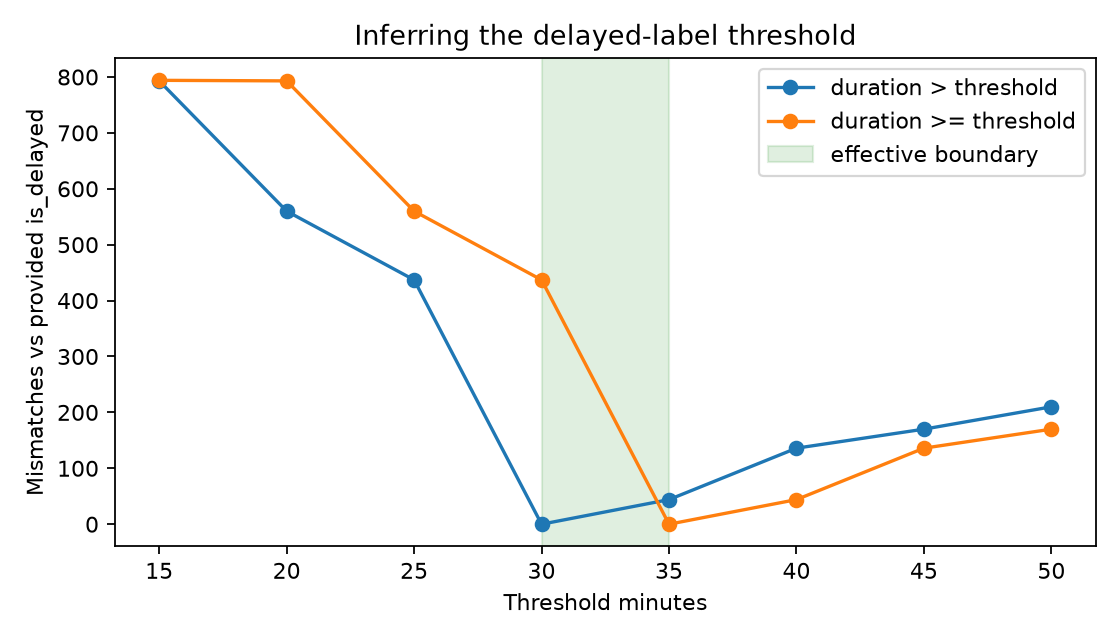
\includegraphics[width=0.74\linewidth]{delay_threshold_inference.png}
\caption{Số mismatch khi thử các luật ngưỡng để phục dựng nhãn trễ.}
\end{figure}

Kết quả này dẫn đến kết luận leakage: các biến sau giao hàng bị cấm trong mô
hình dự báo vì chúng chứa trực tiếp hoặc gián tiếp thông tin tạo ra nhãn:

\begin{itemize}[leftmargin=*]
  \item \code{delivery\_time};
  \item \code{delivery\_duration\_min};
  \item \code{delivery\_efficiency\_min\_per\_km};
  \item \code{delay\_min};
  \item \code{restaurant\_avg\_time}.
\end{itemize}

Feature set chính chỉ dùng biến có thể biết trước khi giao: khoảng cách, số
topping, giờ đặt, size encoding, nhà hàng, địa điểm, loại pizza, traffic,
payment category, peak hour, weekend và tháng đặt hàng.

\section{Data realism và reverse-engineering}

Dataset có nhiều dấu hiệu được tạo bằng hàm sinh dữ liệu hơn là log vận hành
thật. Bảng~\ref{tab:realism} tóm tắt các phát hiện chính.

\begin{table}[H]
\centering
\caption{Dấu hiệu dữ liệu synthetic}
\label{tab:realism}
\begin{tabularx}{\textwidth}{p{4.2cm}X}
\toprule
Kiểm tra & Phát hiện\\
\midrule
Missing value & Không có ô thiếu, bất thường với dữ liệu vận hành thực tế.\\
Thời gian & File tên 2024--25 nhưng \code{order\_time} kéo tới 2026-07-07.\\
Duration & Chỉ có 8 giá trị: 15, 20, 25, 30, 35, 40, 45, 50.\\
Công thức tất định & 7 công thức/target khớp tuyệt đối, gồm estimated duration,
topping density, complexity, traffic impact, delay, efficiency và target.\\
Categorical artifact & Location và pizza type còn tín hiệu mạnh sau khi kiểm
soát distance band.\\
Brand & Count từng brand 194--212 nhưng homogeneity tests không ủng hộ kết luận
các brand đồng nhất thống kê.\\
\bottomrule
\end{tabularx}
\end{table}

\subsection{Cách phát hiện bảy công thức tất định}

Các công thức tất định không được giả định trước. Nhóm dùng quy trình phục dựng:
đọc tên cột và quan hệ nghiệp vụ có khả năng xảy ra, đề xuất biểu thức ứng
viên, tính biểu thức đó trên toàn bộ 1.004 dòng, sau đó đo sai số lớn nhất
giữa cột gốc và biểu thức. Một công thức chỉ được xem là khớp tuyệt đối khi
\code{max\_abs\_error = 0}.

\begin{table}[H]
\centering
\small
\caption{Các công thức tất định được phục dựng}
\begin{tabularx}{\textwidth}{p{3.2cm}p{4.2cm}X}
\toprule
Cột & Công thức khớp & Cách tìm và kiểm chứng\\
\midrule
\code{estimated\_duration\_min} & \code{2.4 * distance\_km} &
Kiểm tra tỷ lệ estimated/distance; tỷ lệ bằng 2,4 cho mọi dòng.\\
\code{topping\_density} & \code{toppings\_count / distance\_km} &
Tên cột gợi ý mật độ; kiểm tra số topping chia cho khoảng cách.\\
\code{pizza\_complexity} & \code{toppings\_count * size\_score} &
Mã hóa Small=1, Medium=2, Large=3, XL=4 rồi nhân với số topping.\\
\code{traffic\_impact} & Low=1, Medium=2, High=3 &
Ba giá trị 1/2/3 khớp một-một với ba mức traffic.\\
\code{delay\_min} & \code{duration - estimated} &
Theo định nghĩa delay hậu nghiệm; kiểm tra duration trừ estimated.\\
\code{delivery\_efficiency} & \code{duration / distance} &
Tên cột là phút/km; kiểm tra duration chia khoảng cách.\\
\code{is\_delayed} & ranh giới giữa 30 và 35 phút &
Thử các luật ngưỡng duration; \code{duration > 30} và
\code{duration >= 35} đều mismatch 0 dòng trên lưới 5 phút.\\
\bottomrule
\end{tabularx}
\end{table}

Kết quả này dẫn tới hai quyết định: các cột hậu nghiệm như duration, delay,
efficiency không được dùng làm feature dự báo; các cột trùng thông tin như
estimated duration, topping density, complexity và traffic impact chỉ dùng để
giải thích/audit, còn mô hình chính dùng feature compact ít trùng lặp hơn.

\begin{figure}[H]
\centering
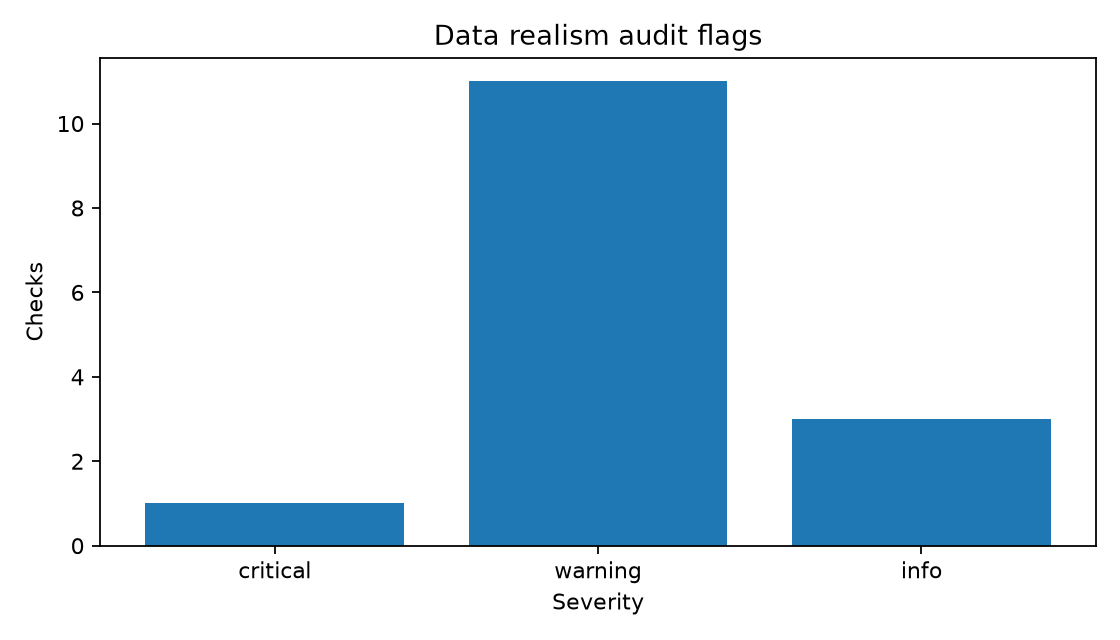
\includegraphics[width=0.74\linewidth]{synthetic_data_flags.png}
\caption{Số lượng cảnh báo trong data realism audit.}
\end{figure}

\begin{figure}[H]
\centering
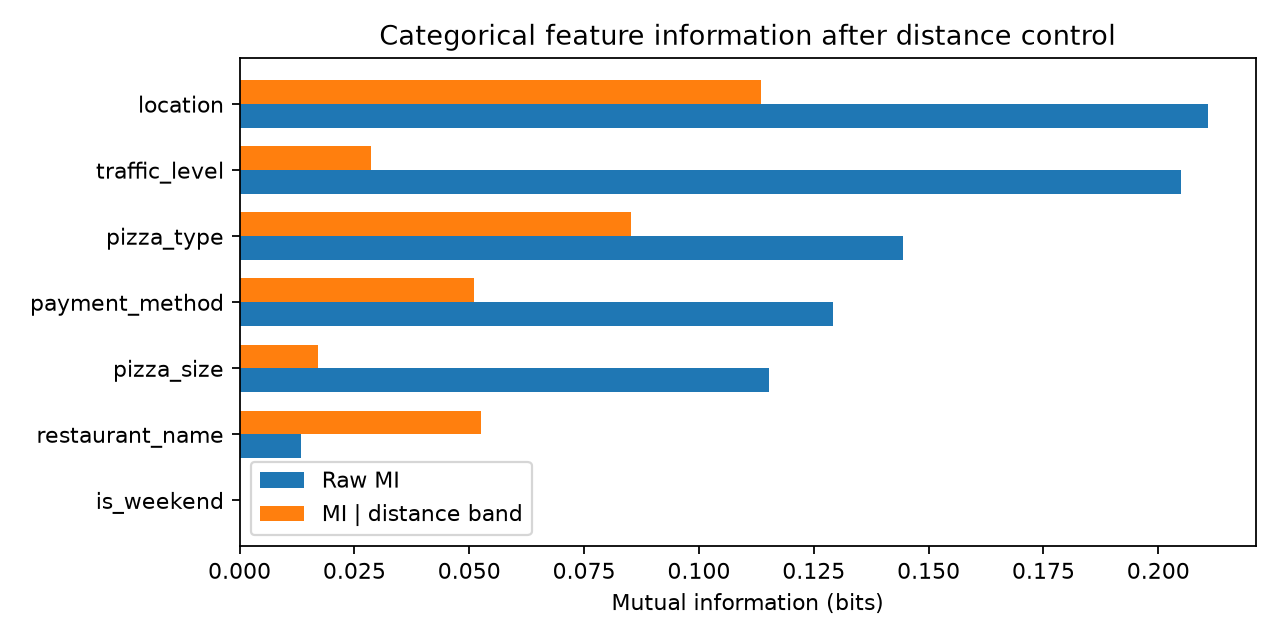
\includegraphics[width=0.82\linewidth]{feature_information_audit.png}
\caption{Mutual information của biến categorical trước và sau khi kiểm soát distance band.}
\end{figure}

\begin{insight}[Ý nghĩa học thuật]
Phần reverse-engineering không nhằm ``sửa'' dataset, mà nhằm đặt giới hạn đúng
cho báo cáo: có thể dùng dữ liệu để minh họa quy trình DSS, nhưng không nên kết
luận rằng brand, location hoặc preference phản ánh thị trường pizza thật.
\end{insight}

\section{Thiết kế split}

Khi thử lấy 20\% cuối theo thời gian, tập test không có mẫu delayed. Vì vậy,
pipeline dùng stratified split cố định để phục vụ đánh giá học thuật.

\begin{table}[H]
\centering
\caption{Split train/dev/test}
\begin{tabular}{lrrr}
\toprule
Split & Số dòng & Delayed & On-time\\
\midrule
Train & 602 & 126 & 476\\
Dev & 201 & 42 & 159\\
Test & 201 & 42 & 159\\
\bottomrule
\end{tabular}
\end{table}

\chapter{Phân tích khám phá và bài toán kinh doanh}

\section{Phân bố nhãn và yếu tố vận hành}

Delayed chiếm 20,92\% nên Accuracy một mình có thể gây hiểu nhầm: baseline
luôn dự báo on-time đã đạt Accuracy 0,7910 nhưng F2 bằng 0 vì bỏ sót toàn bộ
đơn trễ.

\begin{figure}[H]
\centering
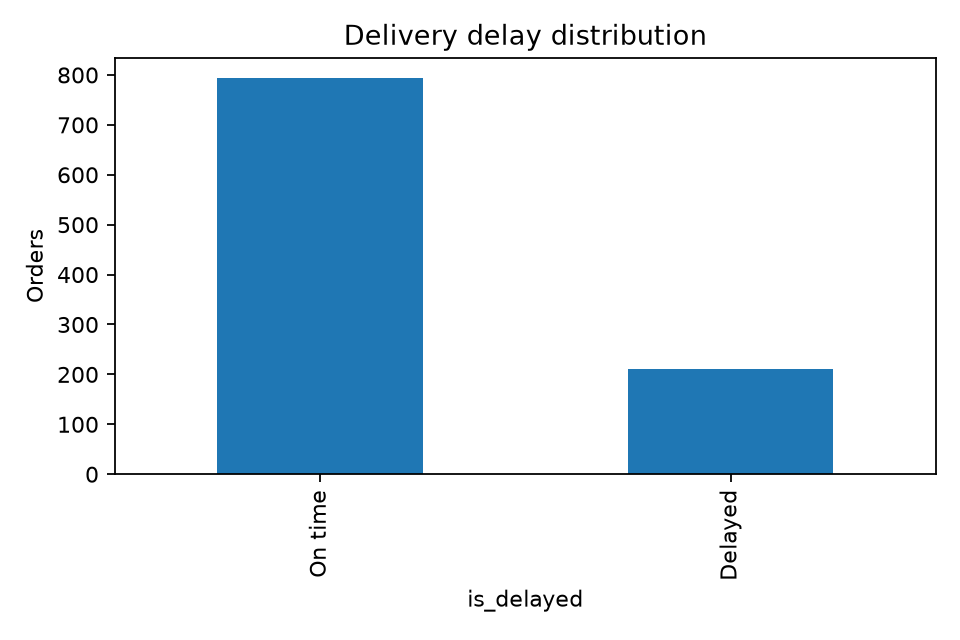
\includegraphics[width=0.68\linewidth]{delay_distribution.png}
\caption{Phân bố đơn đúng giờ và đơn trễ.}
\end{figure}

\subsection{Độ trễ và severity}

Phân tích duration được dùng để hiểu nhãn và mức độ trễ, không dùng làm feature
dự báo. Nhóm on-time có duration trung bình 26,27 phút, trung vị 30 phút và
giá trị lớn nhất 30 phút. Nhóm delayed có duration trung bình 41,67 phút, trung
vị 40 phút và giá trị nhỏ nhất 35 phút. Vì duration chỉ có các mốc 15, 20,
25, 30, 35, 40, 45, 50, nhãn trễ có ranh giới quan sát giữa 30 và 35 phút.

\begin{figure}[H]
\centering
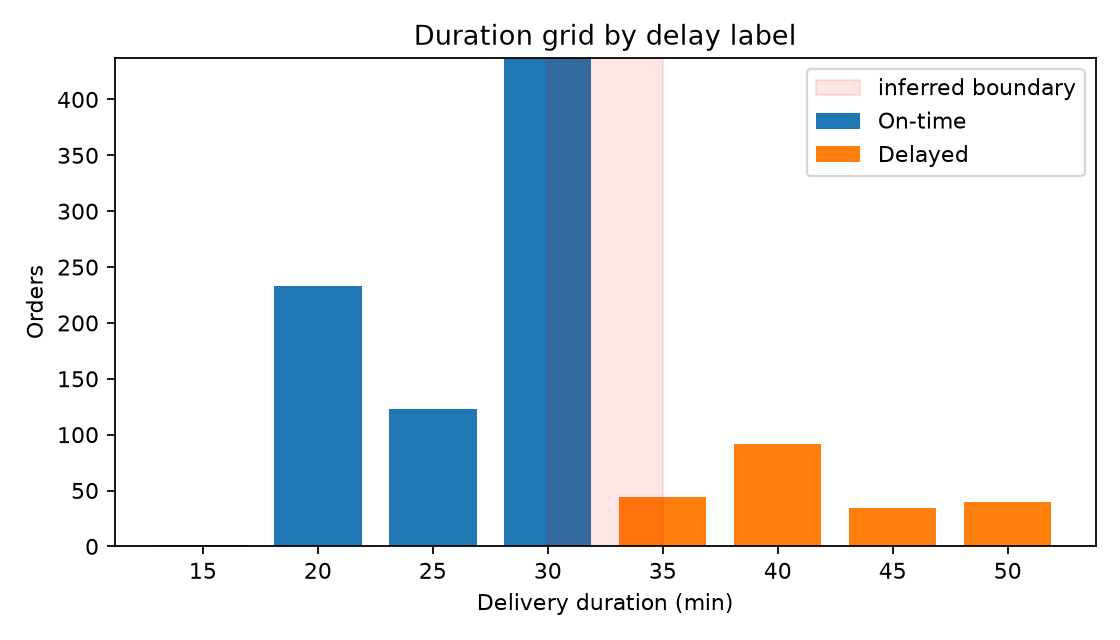
\includegraphics[width=0.72\linewidth]{duration_grid_by_delay.png}
\caption{Duration theo lưới 5 phút và nhãn trễ.}
\end{figure}

\begin{table}[H]
\centering
\caption{Severity của đơn trễ}
\begin{tabular}{lrrrr}
\toprule
Bucket & Orders & Delayed & Avg distance & High traffic share\\
\midrule
On-time <=30 & 794 & 0 & 4,20 & 20,53\%\\
Late 35 & 44 & 44 & 5,52 & 9,09\%\\
Late 40 & 92 & 92 & 7,57 & 97,83\%\\
Late 45--50 & 74 & 74 & 9,35 & 95,95\%\\
\bottomrule
\end{tabular}
\end{table}

Điểm đáng chú ý là nhóm Late 40 và Late 45--50 gần như luôn đi với traffic cao,
trong khi Late 35 lại có high-traffic share thấp. Điều này cho thấy generator
có nhiều luật khác nhau, không chỉ một quan hệ tuyến tính đơn giản.

Traffic và khoảng cách là hai biến có ý nghĩa vận hành rõ nhất. Chúng được giữ
trong feature set compact và cũng được dùng trong công thức Risk Score ở tầng
DSS.

\begin{figure}[H]
\centering
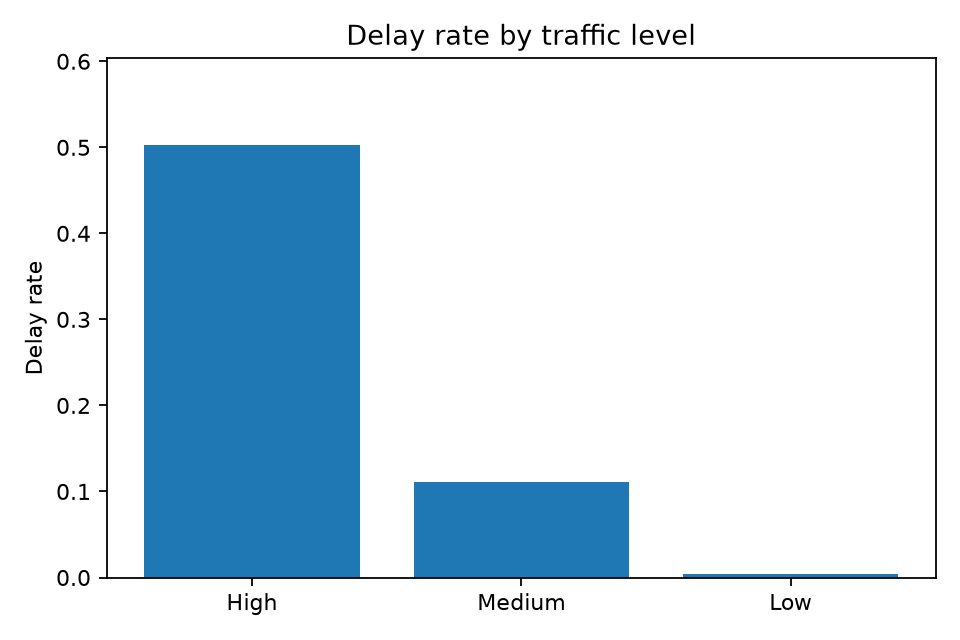
\includegraphics[width=0.68\linewidth]{delay_rate_by_traffic.png}
\caption{Tỷ lệ trễ theo traffic level.}
\end{figure}

\begin{figure}[H]
\centering
\begin{subfigure}{0.48\linewidth}
\centering
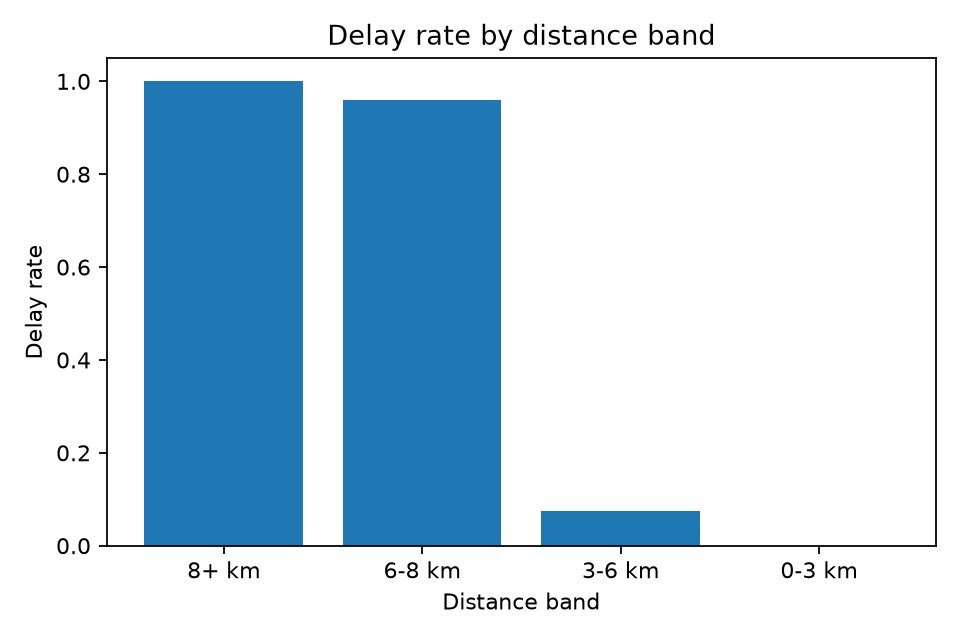
\includegraphics[width=\linewidth]{delay_rate_by_distance_band.png}
\caption{Theo khoảng cách}
\end{subfigure}\hfill
\begin{subfigure}{0.48\linewidth}
\centering
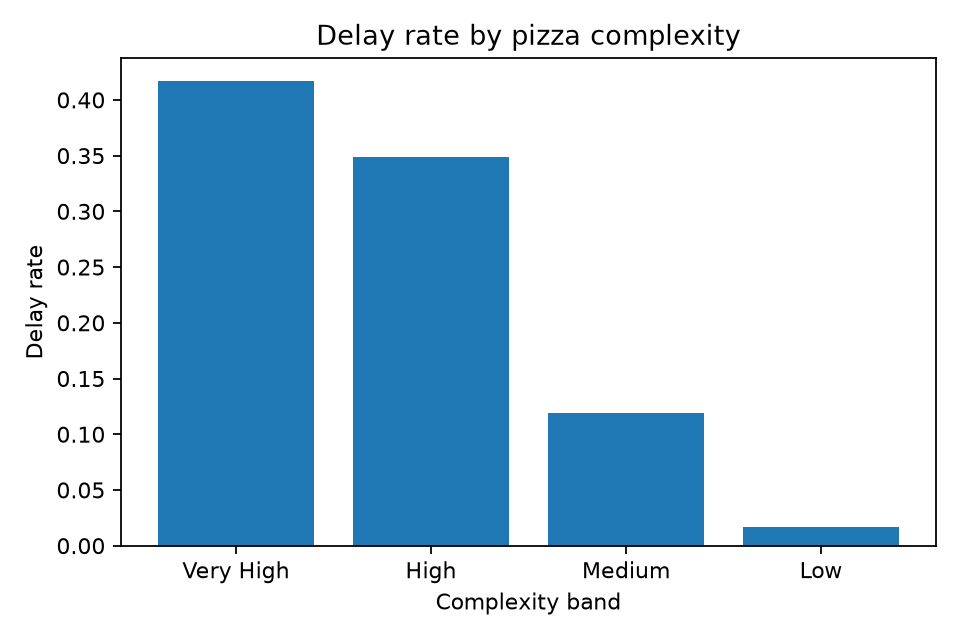
\includegraphics[width=\linewidth]{delay_rate_by_complexity_band.png}
\caption{Theo complexity}
\end{subfigure}
\caption{Tỷ lệ trễ theo các yếu tố vận hành chính.}
\end{figure}

\section{Customer behavior}

Phân tích hành vi khách hàng được dùng cho reporting và recommendation rule,
không dùng làm bằng chứng thị trường thật do dữ liệu synthetic.

\begin{itemize}[leftmargin=*]
  \item Size được chọn nhiều nhất: Medium.
  \item Pizza type được chọn nhiều nhất: Non-Veg.
  \item Cheese Burst ít đơn hơn Non-Veg/Veg nhưng delay rate cao hơn.
  \item Large và XL có delay rate cao hơn Medium/Small.
  \item \code{toppings\_count} chỉ nằm trong 1--5, tập trung ở 2--5.
  \item Location có tín hiệu nhưng nhiều nhóm nhỏ, cần gộp hoặc đọc theo top-location.
\end{itemize}

\begin{figure}[H]
\centering
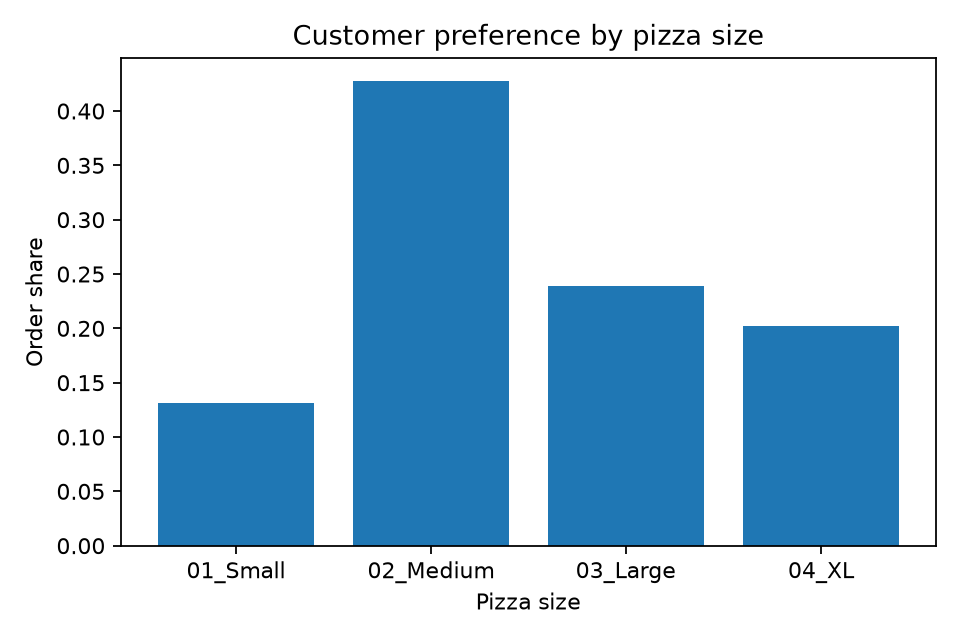
\includegraphics[width=0.66\linewidth]{size_preference.png}
\caption{Tỷ lệ đơn hàng theo size.}
\end{figure}

\begin{figure}[H]
\centering
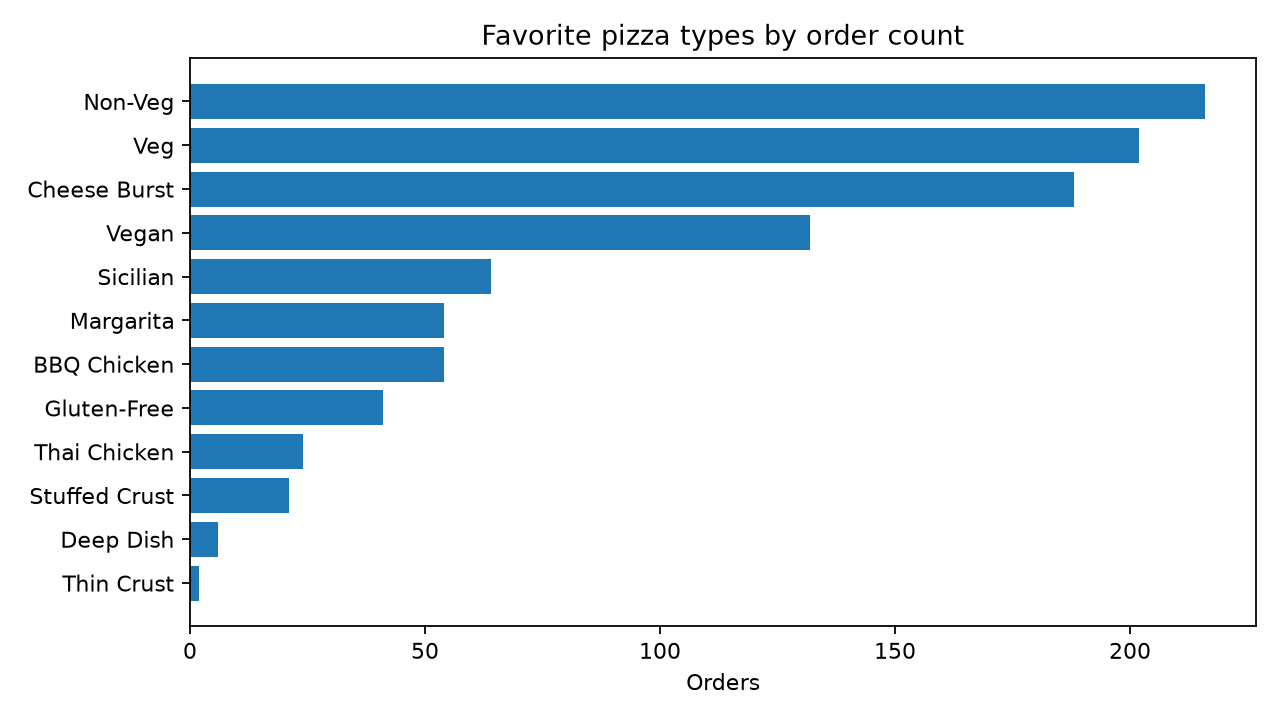
\includegraphics[width=0.78\linewidth]{top_pizza_types.png}
\caption{Các loại pizza được đặt nhiều nhất.}
\end{figure}

\begin{figure}[H]
\centering
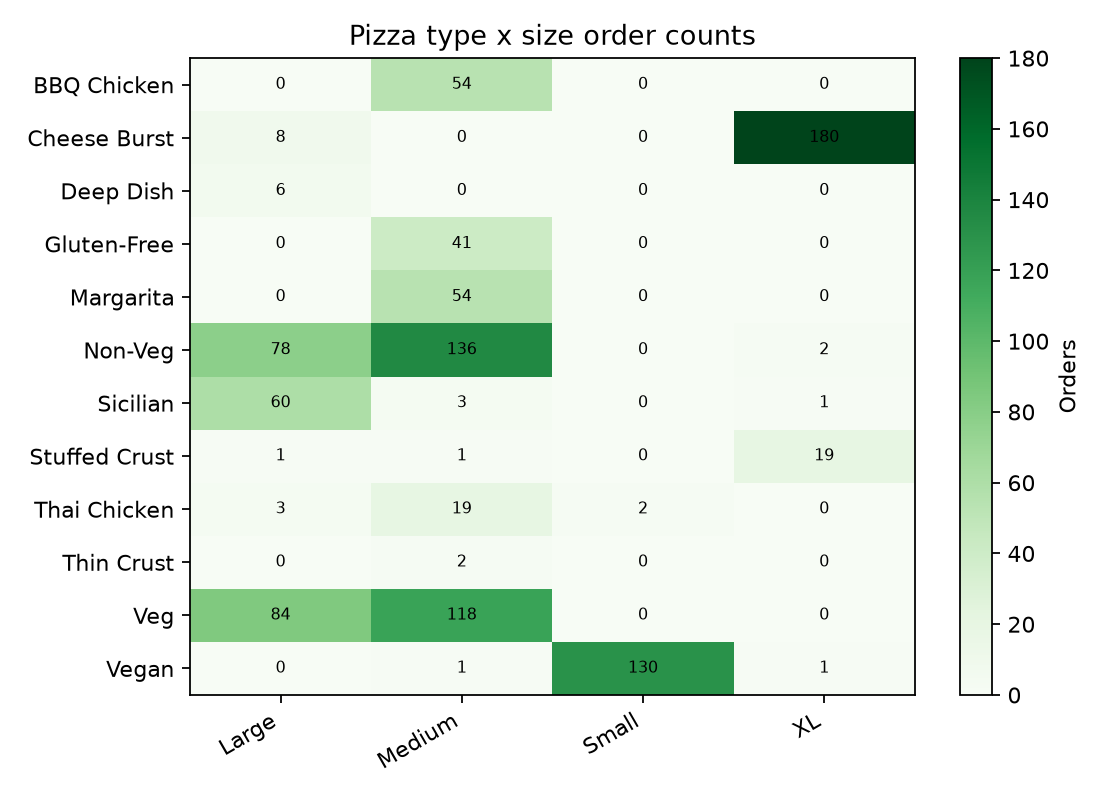
\includegraphics[width=0.74\linewidth]{pizza_type_size_heatmap.png}
\caption{Ma trận số đơn theo pizza type và size.}
\end{figure}

\begin{table}[H]
\centering
\small
\caption{Một số preference và rủi ro nổi bật}
\begin{tabular}{lrrr}
\toprule
Nhóm & Orders & Share & Delay rate\\
\midrule
Non-Veg & 216 & 21,51\% & 20,83\%\\
Veg & 202 & 20,12\% & 21,78\%\\
Cheese Burst & 188 & 18,73\% & 35,64\%\\
Medium & 429 & 42,73\% & 9,09\%\\
Large & 240 & 23,90\% & 35,42\%\\
XL & 203 & 20,22\% & 41,38\%\\
\bottomrule
\end{tabular}
\end{table}

\begin{figure}[H]
\centering
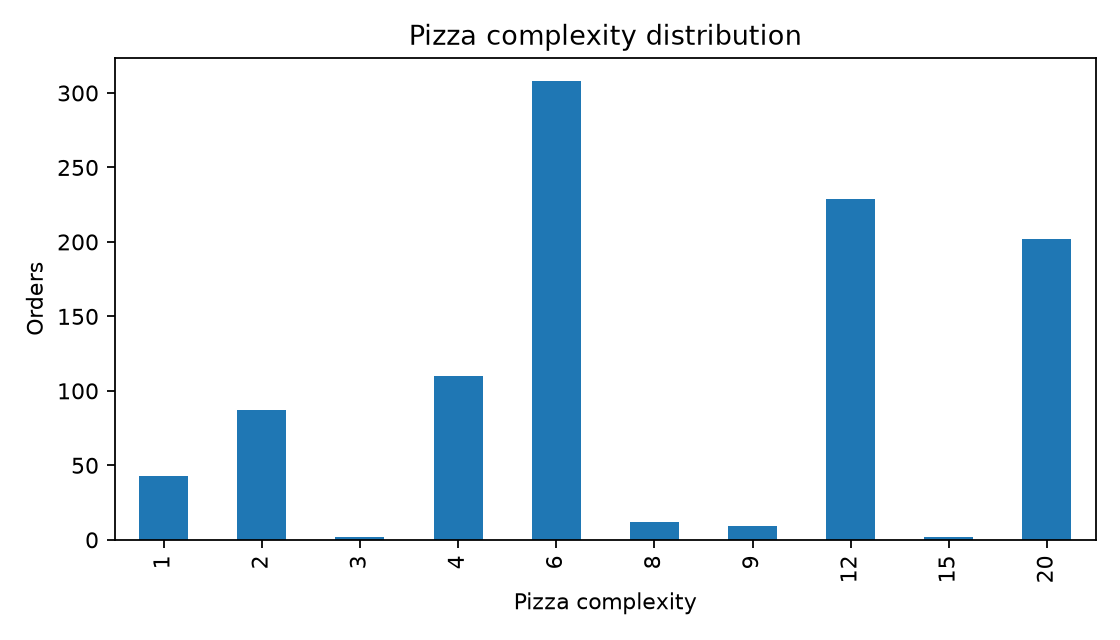
\includegraphics[width=0.66\linewidth]{complexity_distribution.png}
\caption{Phân phối độ phức tạp pizza.}
\end{figure}

\section{Phụ thuộc theo brand, location và state}

Dataset không có cột ``bang'' riêng. Tuy nhiên, \code{location} thường có dạng
\code{City, ST}, nên nhóm tách thêm \code{state\_code} để phân tích mô tả. Đây
không phải geocoding chính thức và chỉ nên đọc như thông tin trong chuỗi
location của dataset.

\begin{figure}[H]
\centering
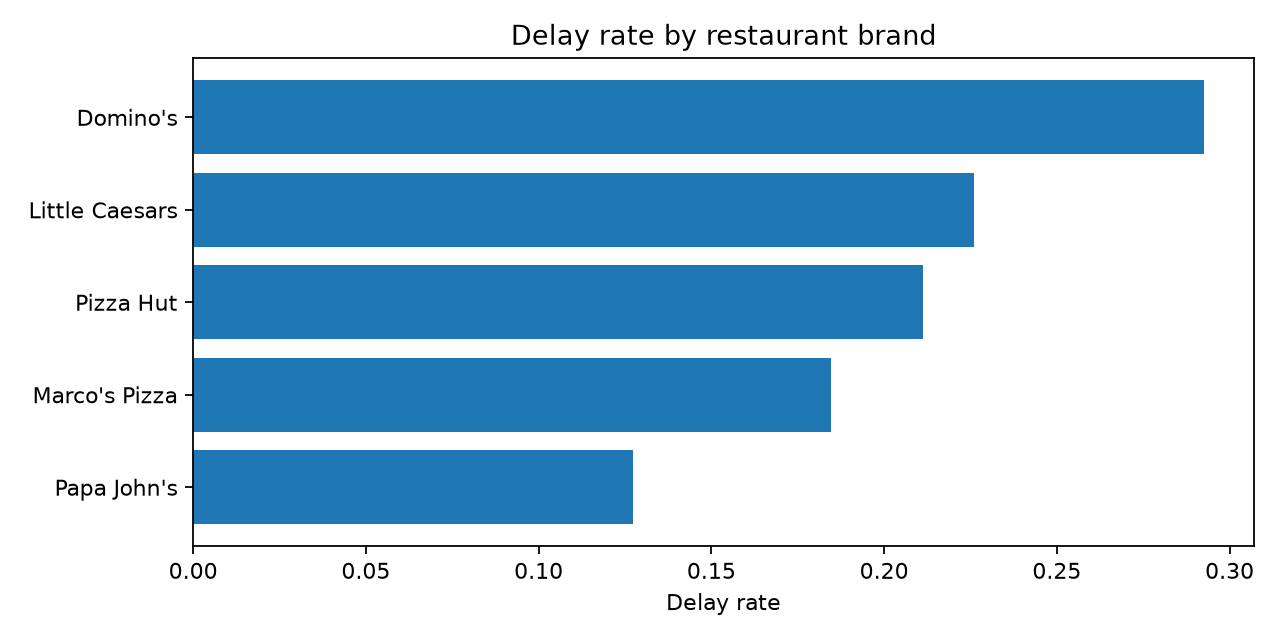
\includegraphics[width=0.78\linewidth]{restaurant_delay_rate.png}
\caption{Delay rate theo restaurant brand.}
\end{figure}

\begin{figure}[H]
\centering
\begin{subfigure}{0.49\linewidth}
\centering
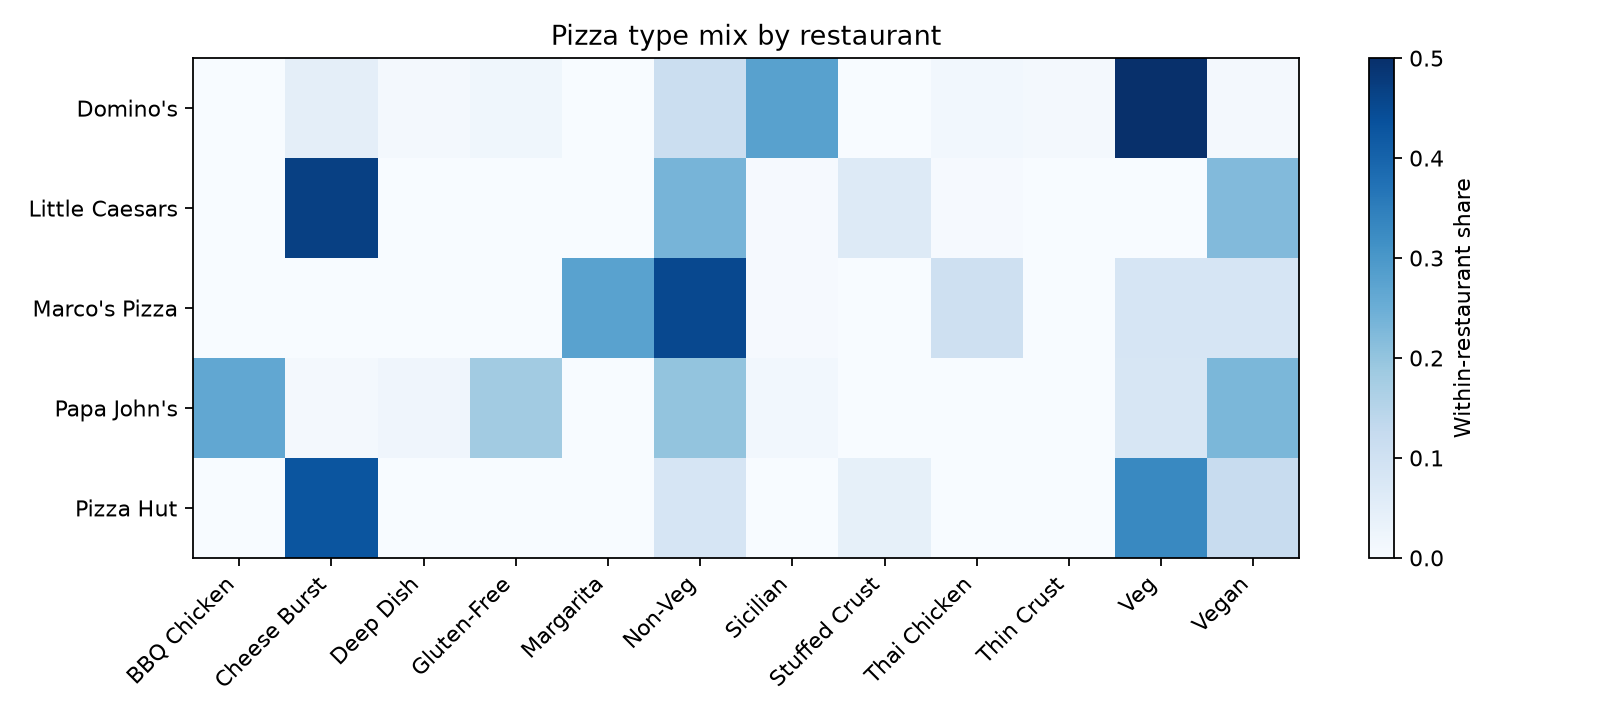
\includegraphics[width=\linewidth]{restaurant_pizza_type_mix_heatmap.png}
\caption{Type mix}
\end{subfigure}\hfill
\begin{subfigure}{0.49\linewidth}
\centering
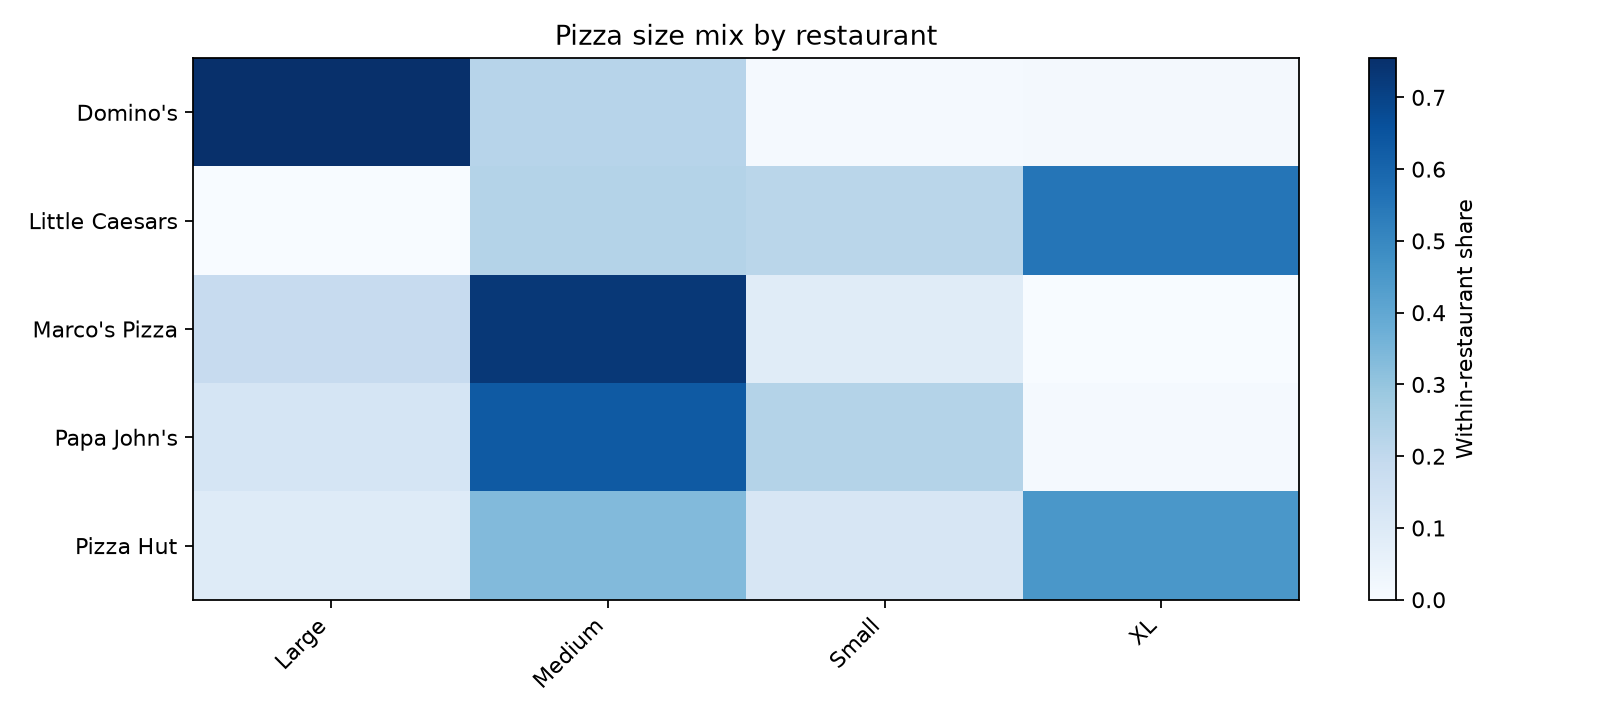
\includegraphics[width=\linewidth]{restaurant_pizza_size_mix_heatmap.png}
\caption{Size mix}
\end{subfigure}
\caption{Cơ cấu sản phẩm theo restaurant brand.}
\end{figure}

\begin{table}[H]
\centering
\small
\caption{Tóm tắt brand}
\begin{tabular}{lrrrr}
\toprule
Brand & Orders & Delay rate & Avg distance & High traffic share\\
\midrule
Domino's & 212 & 29,25\% & 5,52 & 31,13\%\\
Papa John's & 204 & 12,75\% & 4,29 & 13,24\%\\
Little Caesars & 199 & 22,61\% & 5,09 & 62,31\%\\
Marco's Pizza & 195 & 18,46\% & 4,91 & 27,18\%\\
Pizza Hut & 194 & 21,13\% & 4,89 & 29,90\%\\
\bottomrule
\end{tabular}
\end{table}

Brand có khác biệt trong mix, distance và traffic. Tuy nhiên, vì phần
forensics cho thấy dữ liệu mang artifact, báo cáo không kết luận brand nào vận
hành tốt hơn thật sự. Brand được dùng để lọc dashboard và phân tích workload.

\begin{figure}[H]
\centering
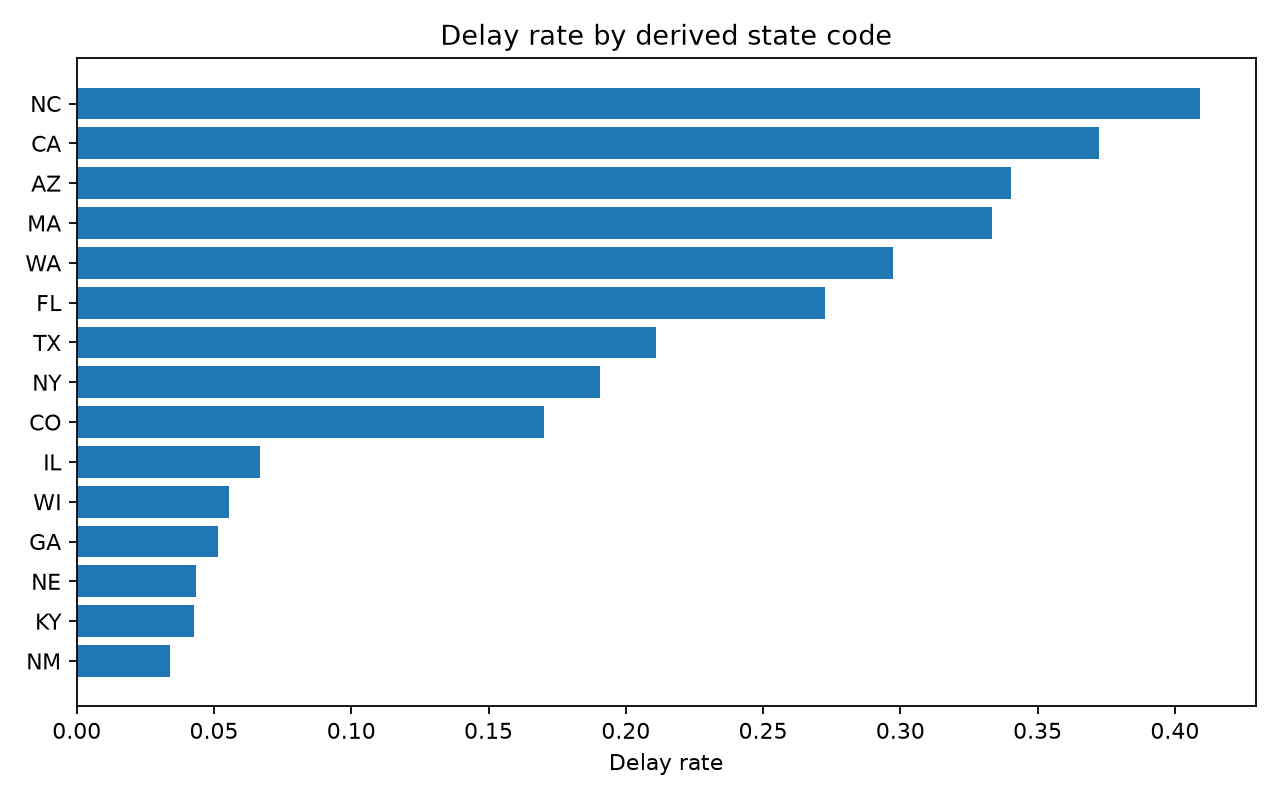
\includegraphics[width=0.76\linewidth]{state_delay_rate_top15.png}
\caption{Delay rate theo state code suy ra từ location.}
\end{figure}

Với location/state, nguyên tắc đọc là luôn nhìn cả số đơn và tỷ lệ trễ. Ví dụ
CA có 94 đơn và delay rate 37,23\%, GA có 78 đơn và delay rate 5,13\%, nhưng
các state nhỏ như OH/IN/TN có tỷ lệ rất cao do mẫu ít. Do đó dashboard nên hiển
thị count, delayed count và small-sample flag thay vì chỉ xếp hạng theo delay
rate.

\section{Kiểm định giả thiết}

Chi-square independence được dùng để kiểm tra mối liên hệ giữa một số biến
categorical và nhãn \code{is\_delayed}. Với mức ý nghĩa 5\%, các biến như
traffic level, pizza type, payment method, complexity band, pizza size,
top-location, restaurant name và time segment cho p-value nhỏ. Tuy nhiên, do
dataset có artifact generator, kết quả được dùng như minh họa phân tích chứ
không suy luận nhân quả.

\section{Forecasting, staffing và recommendation}

Monthly demand được dự báo 6 tháng tới bằng seasonal-naive prior-year. Backtest
có 19 tháng, MAE 12,211 đơn và MAPE 45,7\%. Sai số này đủ lớn để khẳng định
forecast chỉ là demo planning.

\begin{figure}[H]
\centering
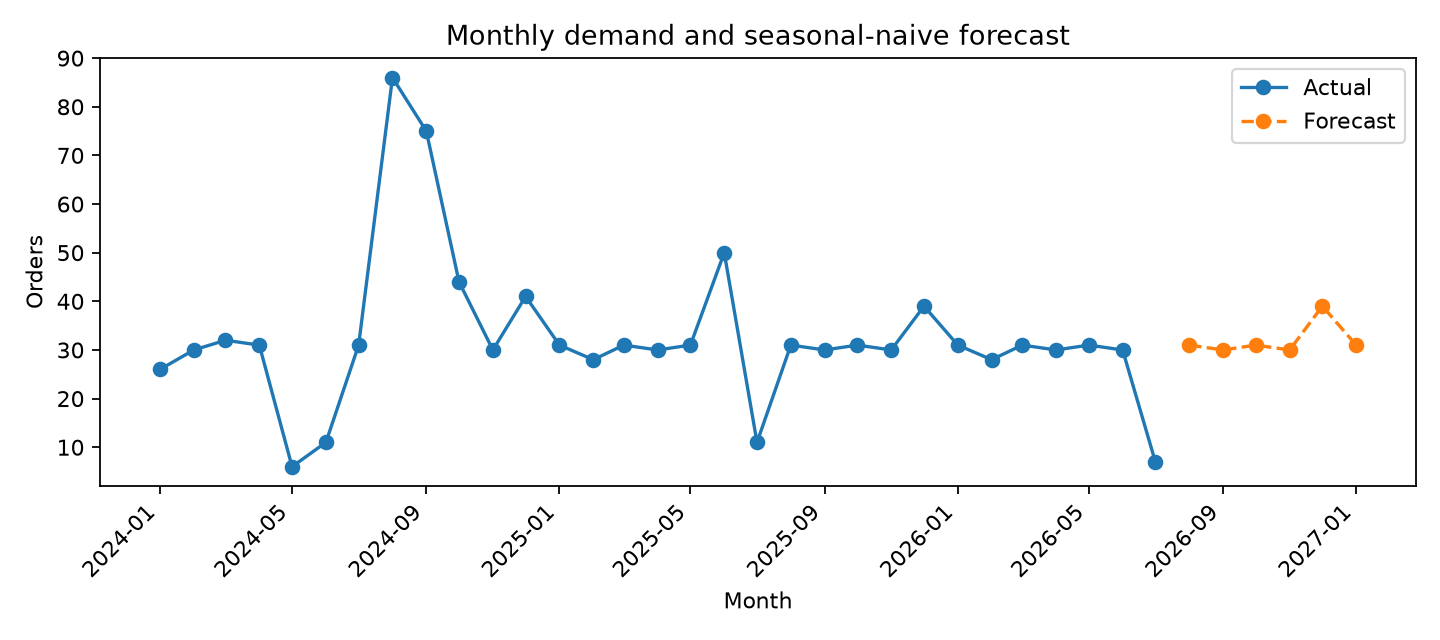
\includegraphics[width=0.78\linewidth]{monthly_demand_forecast.png}
\caption{Nhu cầu theo tháng và dự báo seasonal-naive.}
\end{figure}

Preference trend forecast được xây dựng cho share size/type theo tháng. Một số
slope có p-value nhỏ, nhưng vì dữ liệu synthetic, kết quả chỉ trả lời câu hỏi
``có thể thiết kế quy trình dự báo trend như thế nào'', không kết luận thị hiếu
thật.

\begin{figure}[H]
\centering
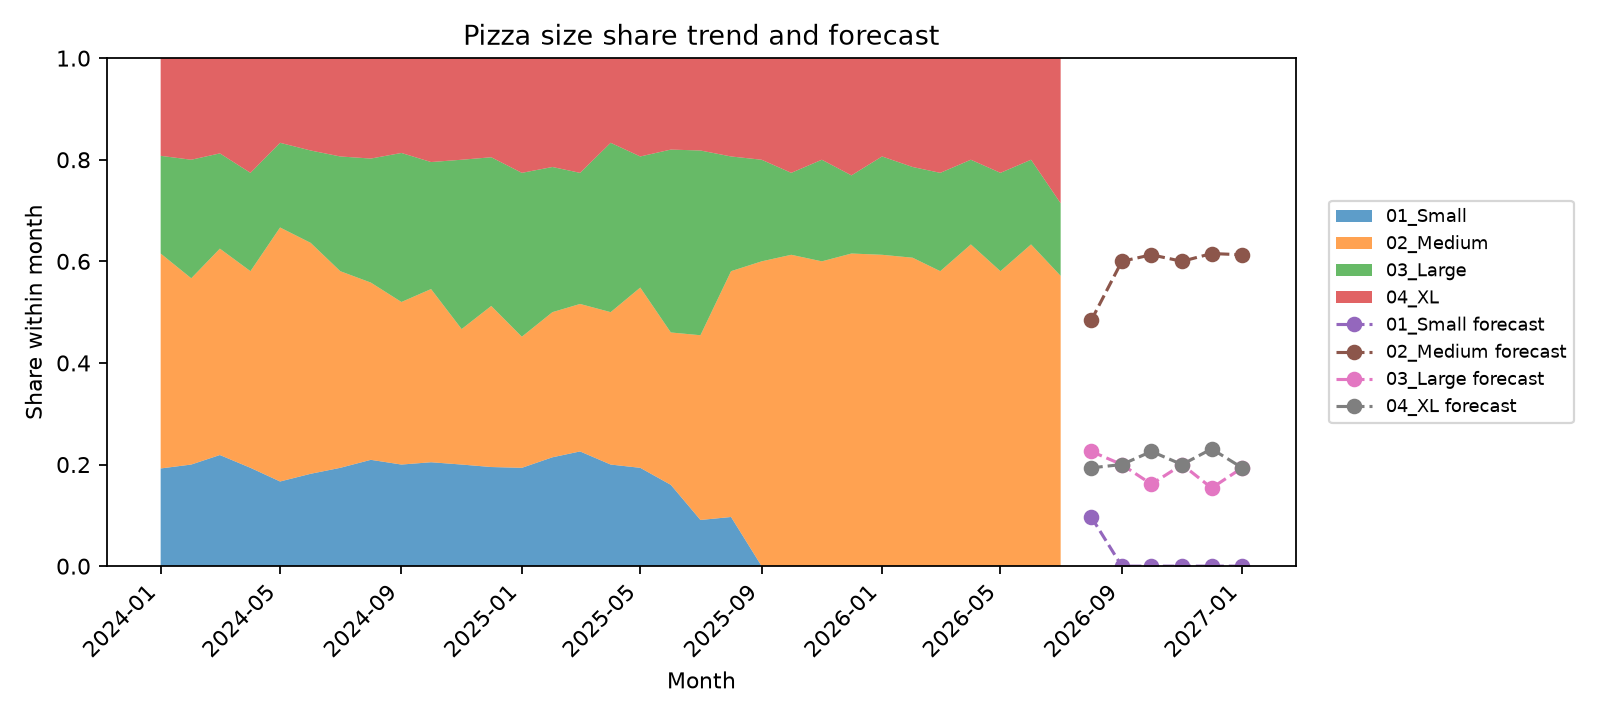
\includegraphics[width=0.78\linewidth]{preference_size_share_forecast.png}
\caption{Forecast share pizza size theo tháng.}
\end{figure}

Với staffing scenario, peak hour là 19h. Bảng \code{hourly\_staffing\_plan.csv}
minh họa cách chuyển phân bố theo giờ thành số nhân sự đề xuất trong kịch bản
100 đơn/ngày.

\chapter{Mô hình dự báo đơn giao trễ}

\section{Thiết kế thực nghiệm}

Mô hình được huấn luyện trên train, chọn trên dev theo F2 và chỉ báo test sau
khi khóa. Preprocessing gồm chuẩn hóa biến số và one-hot encoding biến
categorical. Pipeline scikit-learn đảm bảo scaler/encoder chỉ fit trên train.

Dự án so sánh sáu thuật toán: Logistic Regression, Decision Tree, Gaussian
Naive Bayes, k-NN, SVM và Random Forest. Feature set compact có 12 feature và
loại các biến công thức/trùng thông tin.

\section{So sánh feature set và model}

\begin{table}[H]
\centering
\caption{So sánh feature set trên dev bằng Logistic Regression}
\begin{tabular}{lrrrrr}
\toprule
Feature set & Số feature & Accuracy & Balanced Acc. & F2 & MCC\\
\midrule
Compact non-redundant & 12 & 0,9701 & 0,9636 & 0,9434 & 0,9117\\
Full pre-dispatch & 17 & 0,9701 & 0,9549 & 0,9286 & 0,9097\\
\bottomrule
\end{tabular}
\end{table}

\begin{table}[H]
\centering
\caption{So sánh mô hình trên dev}
\begin{tabular}{lrrrr}
\toprule
Model & Accuracy & Balanced Acc. & F2 & MCC\\
\midrule
Logistic Regression & 0,9701 & 0,9636 & 0,9434 & 0,9117\\
SVM & 0,9602 & 0,9398 & 0,9048 & 0,8796\\
Decision Tree & 0,9502 & 0,9335 & 0,8962 & 0,8525\\
Random Forest & 0,9652 & 0,9254 & 0,8780 & 0,8926\\
k-NN & 0,9353 & 0,8540 & 0,7538 & 0,7970\\
Naive Bayes & 0,6368 & 0,7179 & 0,6642 & 0,3544\\
\bottomrule
\end{tabular}
\end{table}

Logistic Regression được chọn vì đạt F2 cao nhất trên dev, đồng thời có cấu
trúc đơn giản và dễ giải thích hơn các mô hình phức tạp trong phạm vi dataset
nhỏ. Gaussian Naive Bayes vẫn được đưa vào so sánh để có baseline xác suất, nhưng
giả định feature độc lập không phù hợp với dữ liệu này: nhiều feature là biến
đổi từ distance/traffic, nên Bayes có Recall khá nhưng Precision thấp, F2 chỉ
0,6642 và MCC 0,3544.

\section{Dò siêu tham số sau khi chọn model}

Sau vòng model selection, dự án chỉ tune Logistic Regression theo nguyên tắc
``select-then-tune'': chọn họ mô hình trước bằng dev/CV, rồi tinh chỉnh họ thắng.
Tune cả sáu mô hình trên dataset nhỏ sẽ làm tăng số lần so sánh và dễ overfit
dev. Logistic Regression cũng là model phù hợp tầng DSS vì cho xác suất ổn định
và hệ số dễ giải thích hơn SVM/RF.

GridSearchCV chạy trên train với Stratified K-Fold, scoring F2, và lưới
\code{C \in \{0.1, 0.3, 1, 3, 10\}} quanh giá trị mặc định \code{C=1.0}. Kết quả
CV tốt nhất là \code{C=0.3}, nhưng khi refit trên train và so lại trên dev,
phiên bản tuned kém default rõ rệt. Vì vậy model khóa vẫn giữ default
\code{C=1.0}; test chỉ được báo sau quyết định này.

\begin{table}[H]
\centering
\caption{So sánh Logistic Regression default và tuned trên dev}
\begin{tabular}{lrrrrr}
\toprule
Biến thể & C & CV F2 mean & Dev F2 & Dev MCC & Quyết định\\
\midrule
Default LR & 1,0 & 0,9387 & 0,9434 & 0,9117 & Giữ\\
Tuned LR & 0,3 & 0,9437 & 0,8894 & 0,8779 & Không dùng\\
\bottomrule
\end{tabular}
\end{table}

\section{Kiểm soát F-beta threshold và split may mắn}

Ngoài việc chọn model theo F2, dự án kiểm tra riêng bước chọn ngưỡng xác suất.
Ngưỡng 0,5 là mặc định kỹ thuật của classifier; nếu mục tiêu vận hành ưu tiên
Recall mạnh hơn, có thể hạ ngưỡng. Việc quét ngưỡng chỉ dùng dev, không dùng
test để chọn policy.

\begin{table}[H]
\centering
\caption{Ngưỡng tốt nhất trên dev theo F1/F2/F3}
\begin{tabular}{lrrrrrr}
\toprule
Metric & Threshold & Precision & Recall & F-beta & FP & FN\\
\midrule
F1 & 0,4400 & 0,9091 & 0,9524 & 0,9302 & 4 & 2\\
F2 & 0,1569 & 0,7778 & 1,0000 & 0,9459 & 12 & 0\\
F3 & 0,1569 & 0,7778 & 1,0000 & 0,9722 & 12 & 0\\
\bottomrule
\end{tabular}
\end{table}

\begin{figure}[H]
\centering
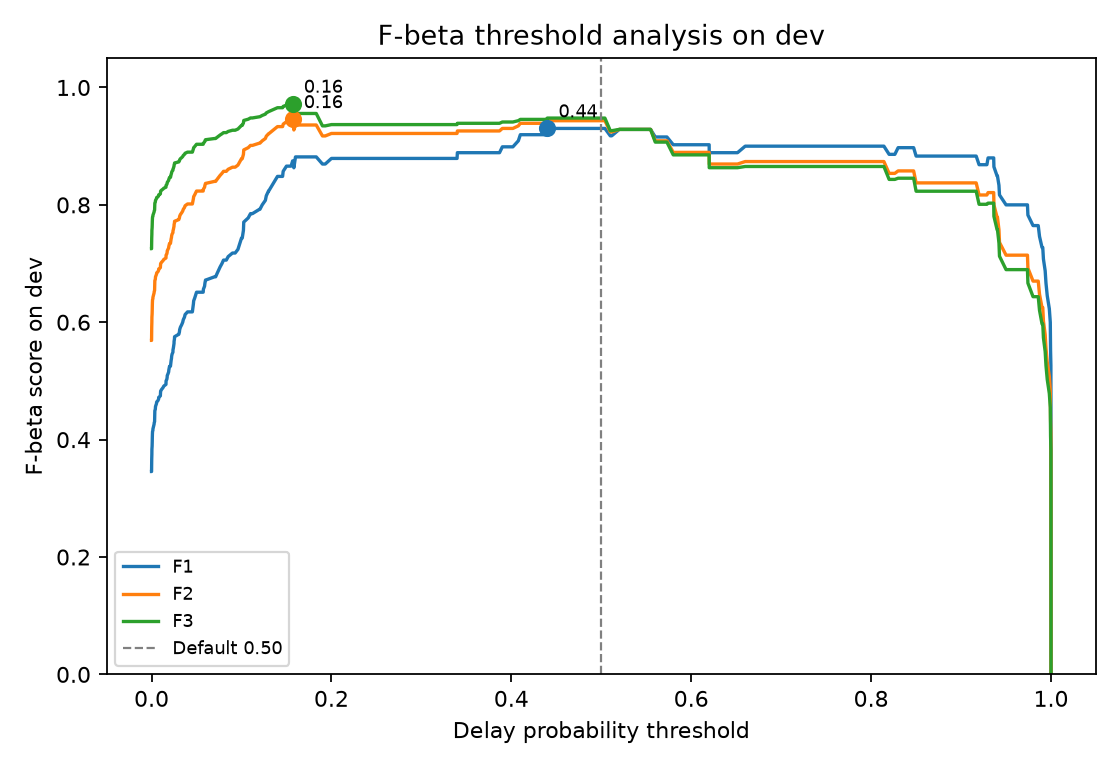
\includegraphics[width=0.78\linewidth]{fbeta_threshold_curve.png}
\caption{Quét ngưỡng F-beta trên dev.}
\end{figure}

Khi chuyển ngưỡng F2 tối ưu từ dev sang test, Recall đạt 1,0 và không còn FN,
nhưng FP tăng từ 7 lên 22; F2 test giảm từ 0,9491 xuống 0,9052. Do đó báo cáo
chính giữ ngưỡng 0,5 cho metric test, còn dashboard coi threshold là policy có
thể chỉnh nếu quản lý muốn đánh đổi thêm FP để giảm FN.

\begin{table}[H]
\centering
\caption{Transfer ngưỡng từ dev sang test}
\begin{tabular}{lrrrrrrr}
\toprule
Policy test & Threshold & Precision & Recall & F1 & F2 & FP & FN\\
\midrule
Default 0,5 & 0,5000 & 0,8542 & 0,9762 & 0,9111 & 0,9491 & 7 & 1\\
Dev-best F2 & 0,1569 & 0,6563 & 1,0000 & 0,7925 & 0,9052 & 22 & 0\\
\bottomrule
\end{tabular}
\end{table}

Để kiểm soát khả năng ``ăn may'' do một split đẹp, dự án còn chạy 100 lần
repeated stratified holdout trên pool train+dev, giữ test ngoài audit. Logistic
Regression được refit ở mỗi run với threshold 0,5. Kết quả cho thấy điểm cao
khá ổn định nhưng vẫn có biên dao động, nên không overclaim con số 0,95 như một
đảm bảo tuyệt đối.

\begin{table}[H]
\centering
\caption{Tóm tắt 100-run stability audit trên train+dev}
\begin{tabular}{lrrrrr}
\toprule
Metric & Mean & Std & Min & P05 & P95\\
\midrule
F2 & 0,9419 & 0,0279 & 0,8416 & 0,8892 & 0,9770\\
MCC & 0,9161 & 0,0290 & 0,8495 & 0,8687 & 0,9569\\
Recall & 0,9481 & 0,0355 & 0,8095 & 0,8810 & 1,0000\\
Precision & 0,9206 & 0,0367 & 0,8200 & 0,8542 & 0,9756\\
\bottomrule
\end{tabular}
\end{table}

\begin{figure}[H]
\centering
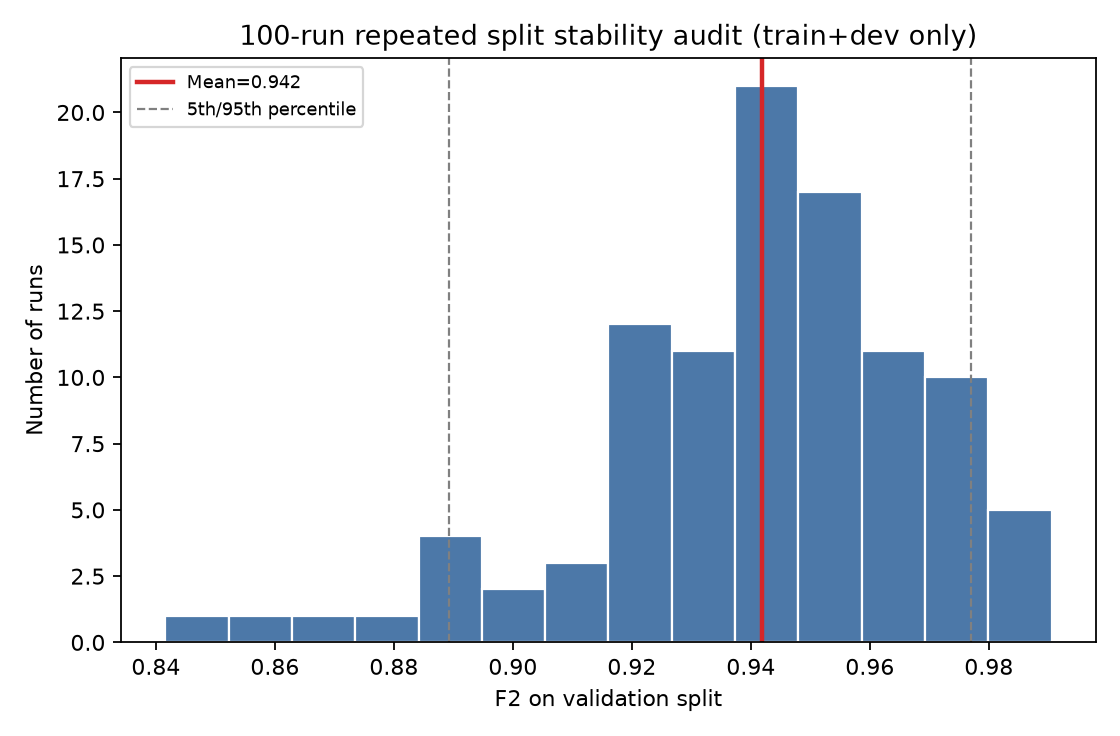
\includegraphics[width=0.78\linewidth]{model_stability_f2_distribution.png}
\caption{Phân phối F2 qua 100 lần chia lại train/dev.}
\end{figure}

\section{Kết quả test và baseline}

\begin{table}[H]
\centering
\caption{Kết quả test của model khóa}
\begin{tabular}{lr}
\toprule
Metric & Giá trị\\
\midrule
Accuracy & 0,9602\\
Balanced Accuracy & 0,9661\\
Precision & 0,8542\\
Recall & 0,9762\\
F1 & 0,9111\\
F2 & 0,9491\\
MCC & 0,8889\\
ROC-AUC & 0,9961\\
\bottomrule
\end{tabular}
\end{table}

\begin{table}[H]
\centering
\caption{Confusion matrix trên test}
\begin{tabular}{lrr}
\toprule
 & Predicted on-time & Predicted delayed\\
\midrule
Actual on-time & 152 & 7\\
Actual delayed & 1 & 41\\
\bottomrule
\end{tabular}
\end{table}

\begin{table}[H]
\centering
\caption{Baseline test}
\begin{tabular}{lrrr}
\toprule
Baseline & Accuracy & F2 & MCC\\
\midrule
Always on-time & 0,7910 & 0,0000 & 0,0000\\
Always delayed & 0,2090 & 0,5691 & 0,0000\\
\bottomrule
\end{tabular}
\end{table}

Kết quả cho thấy mô hình khóa vượt hai baseline trên các metric cân bằng. Tuy
nhiên, vì target được sinh từ ngưỡng duration và dữ liệu có tính synthetic, kết
quả này không nên được quảng bá như hiệu năng sản xuất.

\chapter{Tầng DSS, dashboard và tối ưu vận tải}

\section{Từ xác suất đến quyết định}

Xác suất delayed không tự nó là quyết định. DSS chuyển xác suất thành Risk
Score bằng cách kết hợp xác suất mô hình với traffic, distance, peak hour,
complexity và weekend:

\[
\begin{aligned}
Risk =&\ 0,55S_{model} + 0,15S_{traffic} + 0,12S_{distance}\\
&+ 0,08S_{peak} + 0,06S_{complexity} + 0,04S_{weekend}.
\end{aligned}
\]

\begin{table}[H]
\centering
\caption{Chuẩn hóa từng thành phần Risk Score}
\small
\begin{tabularx}{\linewidth}{lrlX}
\toprule
Thành phần & Weight & Công thức điểm 0--100 & Lý do\\
\midrule
\(S_{model}\) & 0,55 & \(P(delayed)\times100\) & Tín hiệu học máy là bằng chứng chính.\\
\(S_{traffic}\) & 0,15 & Low=20, Medium=60, High=100 & Traffic là driver vận hành rõ trong EDA.\\
\(S_{distance}\) & 0,12 & \(\min(distance/10\times100,100)\) & 10 km là mức xa nhất trong dữ liệu.\\
\(S_{peak}\) & 0,08 & Peak=100, non-peak=20 & Giờ cao điểm ảnh hưởng năng lực xử lý.\\
\(S_{complexity}\) & 0,06 & \(\min(complexity/20\times100,100)\) & Complexity tối đa quan sát là 20.\\
\(S_{weekend}\) & 0,04 & Weekend=70, weekday=40 & Tín hiệu phụ, weight nhỏ vì audit yếu.\\
\bottomrule
\end{tabularx}
\end{table}

Các trọng số cộng đúng 1,0 và được chọn như một policy minh bạch: mô hình chiếm
vai trò chính, còn traffic/distance/peak/complexity/weekend là áp lực vận hành
để người điều phối hiểu vì sao một đơn được đẩy lên hàng đợi. Đây không phải
trọng số tối ưu thống kê; nếu cửa hàng đổi năng lực xử lý, policy có thể chỉnh.

\begin{figure}[H]
\centering
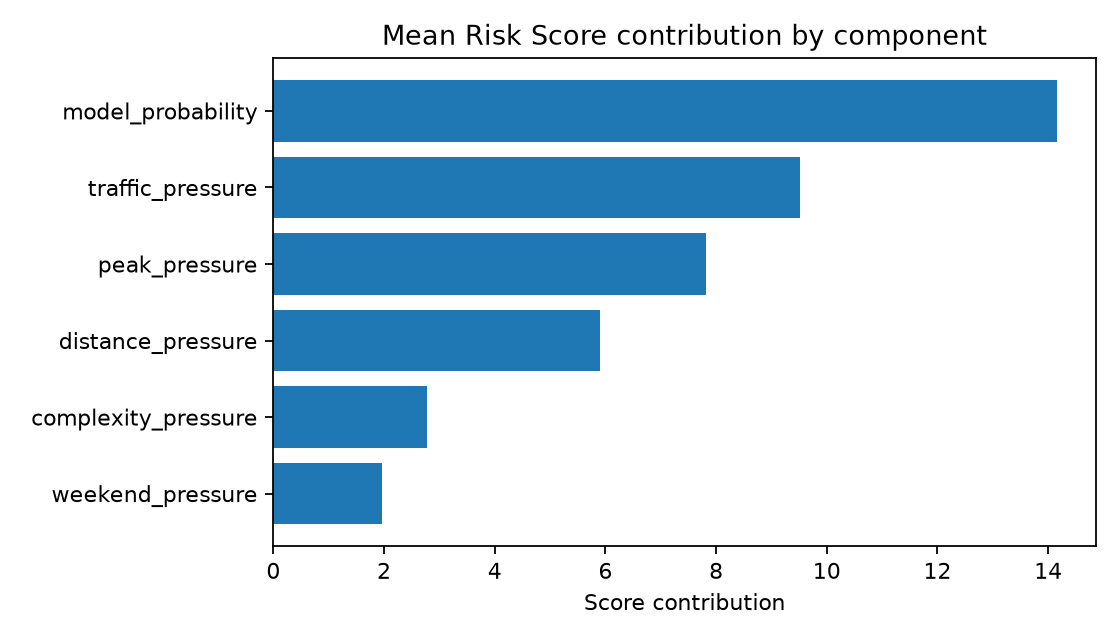
\includegraphics[width=0.78\linewidth]{risk_component_breakdown.png}
\caption{Đóng góp trung bình của từng thành phần vào Risk Score.}
\end{figure}

Risk Score được ánh xạ thành Priority:

\begin{table}[H]
\centering
\caption{Ngưỡng priority}
\begin{tabular}{rl}
\toprule
Risk Score & Priority\\
\midrule
0--35 & Low\\
36--65 & Medium\\
66--100 & High\\
\bottomrule
\end{tabular}
\end{table}

Recommended Action tương ứng:

\begin{itemize}[leftmargin=*]
  \item High: báo điều phối trưởng, chuẩn bị tài xế dự phòng, thông báo customer support.
  \item Medium: theo dõi tài xế/traffic, cập nhật khách hàng nếu ETA xấu đi.
  \item Low: giữ trong hàng đợi bình thường.
\end{itemize}

\begin{figure}[H]
\centering
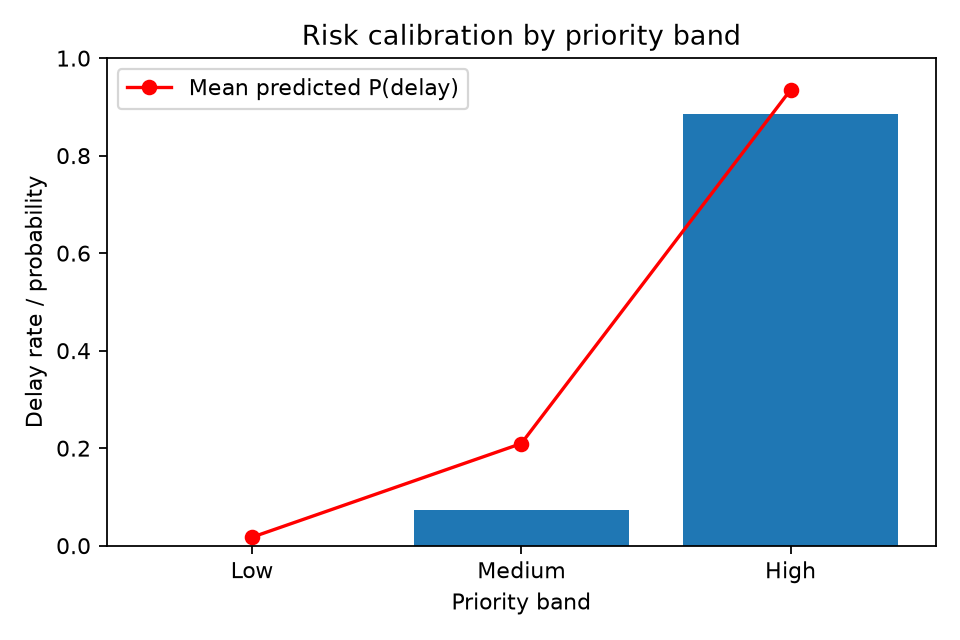
\includegraphics[width=0.78\linewidth]{risk_calibration.png}
\caption{Calibration: delay rate thực tế theo priority band.}
\end{figure}

\begin{figure}[H]
\centering
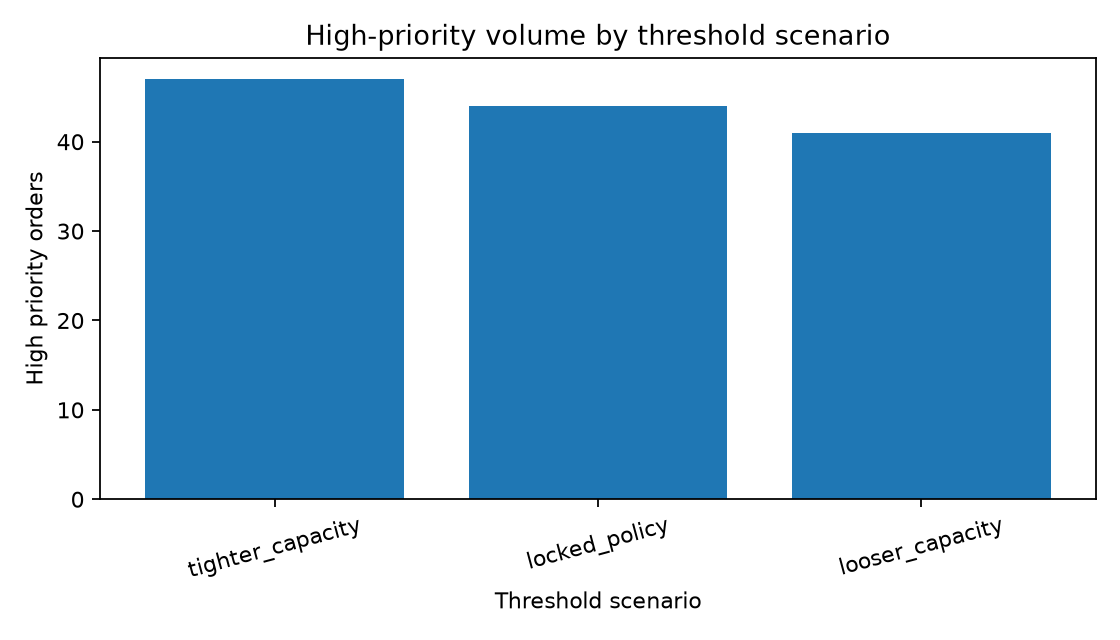
\includegraphics[width=0.78\linewidth]{priority_threshold_sensitivity.png}
\caption{Độ nhạy số đơn High priority khi thay ngưỡng.}
\end{figure}

Calibration cho thấy delay rate tăng từ Low 0,0\% sang Medium 7,3\% và High
88,6\%. Ngưỡng 35/65 được giữ như policy khóa vì bắt được 92,9\% đơn trễ trong
nhóm High, nhưng sensitivity chứng minh đây là tham số vận hành, không phải
chân lý tuyệt đối.

\section{Kịch bản assignment}

Dự án lấy nhóm đơn High priority từ queue, tạo fleet tài xế giả lập có capacity
và tối thiểu hóa chi phí gán đơn--tài xế. Kết quả hiện tại gán 12 đơn High
priority cho 6 tài xế giả lập, mean assignment cost 32,84. Đây là minh họa tầng
prescriptive DSS vì dataset Kaggle không có depot, driver logs hoặc capacity
thật.

\begin{table}[H]
\centering
\small
\caption{Minh bạch công thức cost trong kịch bản assignment}
\begin{tabularx}{\textwidth}{p{3.4cm}p{5.6cm}X}
\toprule
Thành phần & Công thức & Nguồn/ý nghĩa\\
\midrule
Travel minutes & \code{distance\_km * 3.2 / speed\_factor} &
\code{distance\_km} đến từ đơn thật; \code{speed\_factor} là giả lập cho tài xế.\\
Priority penalty & \code{0.35 * (100 - delay\_risk\_score)} &
Đơn risk càng cao thì penalty càng thấp, nên được ưu tiên trong tối ưu.\\
High traffic penalty & \code{6 nếu traffic = High} &
Traffic cao cần thêm buffer vận hành.\\
Same-location bonus & \code{-8 nếu cùng location/base} &
Ưu tiên tài xế cùng khu vực trong fleet giả lập.\\
Cost floor & \code{max(total, 0)} &
Đảm bảo cost không âm khi có bonus.\\
\bottomrule
\end{tabularx}
\end{table}

Thuật toán chính là Hungarian linear-sum assignment nếu \code{scipy} khả dụng;
greedy chỉ là fallback để pipeline vẫn chạy trong môi trường thiếu thư viện.
Vì cost dùng proxy và fleet giả lập, phần này chỉ chứng minh cách biến queue
thành khuyến nghị phân công, không phải claim tối ưu điều phối tài xế thật.

\section{Dashboard Streamlit và Power BI}

Dashboard Streamlit gồm tám tab: Overview, EDA, Customer Behavior, Forecast \&
Staffing, Model Evaluation, Single Order Demo, Delay Queue và Data Quality.
Dashboard giúp người dùng xem KPI, giải thích mô hình, thử một đơn mới, xem
hàng đợi ưu tiên, bóc tách Risk Score và kiểm tra kịch bản assignment.

Power BI pack gồm fact/dim CSV, DAX measures và dashboard spec. Dự án không tự
sinh file \code{.pbix}; nếu lớp yêu cầu dashboard native, cần import các bảng
CSV vào Power BI Desktop theo hướng dẫn trong thư mục \code{powerbi/}.

\chapter{Minh chứng tái lập và đánh giá dự án}

\section{Runbook và kiểm thử}

Runbook chính:

\begin{verbatim}
cd pizza_delivery_dss
python -m scripts.run_all
python -m unittest discover -s tests -v
streamlit run app/streamlit_app.py
\end{verbatim}

Pipeline \code{scripts.run\_all} gồm 18 bước, từ audit dữ liệu đến build
notebook, report PDF, slide PDF, unit tests và Streamlit smoke test. Kiểm thử
hiện tại gồm 30 unit tests cho schema, leakage, split, detailed EDA, forensics, brand
ablation, preference forecast, model, cross-validation, bootstrap CI, DSS rules
và assignment.

\section{Đối chiếu yêu cầu học phần}

\begin{table}[H]
\centering
\small
\caption{Đối chiếu nội dung học phần với dự án}
\begin{tabularx}{\textwidth}{p{4.0cm}X}
\toprule
Nội dung & Thể hiện trong dự án\\
\midrule
DSS & Predictive layer, Risk Score, Priority, dashboard.\\
Supervised learning & Dự báo \code{is\_delayed}.\\
Decision Tree, Naive Bayes, k-NN, SVM, Ensemble & Được so sánh trong Chương 5.\\
Evaluation & Train/dev/test, baseline, F2, Balanced Accuracy, MCC.\\
Hypothesis testing & Chi-square cho biến categorical.\\
Clustering/association & K-Means và association rules trong EDA.\\
Time series & Monthly demand forecast và preference share forecast.\\
Recommendation & Popularity/context rules.\\
Optimization & Assignment scenario cho đơn High priority.\\
BI/dashboard & Streamlit và Power BI-ready pack.\\
\bottomrule
\end{tabularx}
\end{table}

\section{Các câu hỏi phản biện đã kiểm soát}

\begin{table}[H]
\centering
\small
\caption{Câu hỏi dễ bị hỏi khi bảo vệ và câu trả lời khóa}
\begin{tabularx}{\textwidth}{p{4.2cm}X}
\toprule
Câu hỏi & Câu trả lời trong dự án\\
\midrule
Sao biết đơn trễ là sau 30 phút? &
Không giả định SLA trước. Nhóm suy luận từ nhãn: on-time max 30 phút, delayed
min 35 phút; vì duration nằm trên lưới 5 phút nên \code{>30} và \code{>=35}
khớp nhãn 0 mismatch.\\
Vì sao không dùng \code{delivery\_duration\_min}? &
Đó là thông tin sau giao hàng và phục dựng nhãn trực tiếp; dùng làm feature sẽ
leakage.\\
Vì sao không chọn Naive Bayes? &
Naive Bayes đã được thử trong 6 classifier nhưng dev F2/MCC thấp hơn rõ; giả
định độc lập feature không hợp với distance, estimated duration, complexity và
các biến được sinh từ nhau.\\
F-beta có được tối ưu không? &
Có quét threshold F1/F2/F3 trên dev. Dev-best F2 bắt hết delayed nhưng transfer
sang test làm FP tăng 7 lên 22 và F2 giảm, nên giữ threshold 0,5 cho báo cáo
chính.\\
Điểm F2 cao có do may mắn split không? &
100-run train+dev stability cho F2 mean 0,9419 và p05 0,8892; điểm cao tương
đối ổn định, nhưng vẫn được giải thích bằng data synthetic/generator gần tất
định, không overclaim production.\\
Risk Score và assignment có tối ưu thống kê không? &
Không. Risk Score là weighted scoring policy minh bạch; assignment dùng cost
proxy và fleet giả lập. Hai phần này là prototype prescriptive DSS, cần SLA,
driver log và cost thật nếu triển khai.\\
Forecast/recommendation dùng được kinh doanh thật không? &
Không claim. Forecast MAPE 45,7\% và recommendation là popularity/context rule,
chỉ minh họa quy trình planning và reporting trên dữ liệu synthetic.\\
\bottomrule
\end{tabularx}
\end{table}

\section{Khuyến nghị ra quyết định}

Chuyển kết quả phân tích thành hành động cụ thể cho quản lý vận hành, kèm điều
kiện áp dụng:

\begin{enumerate}[leftmargin=*]
  \item \textbf{Ưu tiên theo Risk Score.} Dùng hàng đợi
        \code{delay\_priority\_queue.csv}: xử lý nhóm High trước (chuẩn bị tài
        xế dự phòng, thông báo khách), nhóm Medium theo dõi traffic/ETA, nhóm
        Low giữ luồng thường. Calibration cho thấy delay-rate thật tăng dần theo
        risk band nên thứ tự ưu tiên này có căn cứ dữ liệu.
  \item \textbf{Tập trung nguồn lực vào đơn xa \& giờ cao điểm.} Distance và
        traffic là yếu tố rủi ro mạnh nhất (EDA + hệ số mô hình); với đơn
        distance lớn và traffic cao nên gán tài xế nhanh/kinh nghiệm.
  \item \textbf{Bố trí nhân sự theo giờ.} Kịch bản staffing cho thấy đỉnh đơn
        quanh 19h; tăng ca giờ cao điểm thay vì rải đều.
  \item \textbf{Ngưỡng Priority là tham số điều chỉnh được.} Đặt ngưỡng 35/65
        theo năng lực xử lý thực tế (phân tích độ nhạy ở Chương 6); nâng ngưỡng
        khi đội mỏng để giảm số đơn phải can thiệp.
  \item \textbf{Điều kiện áp dụng.} Các khuyến nghị trên là cơ chế hỗ trợ minh
        bạch trên dữ liệu hiện có; trước khi dùng thật cần log vận hành thật,
        chi phí SLA và đánh giá theo thời gian (xem Giới hạn).
\end{enumerate}

\section{Giới hạn}

\begin{enumerate}[leftmargin=*]
  \item Dataset nhỏ và có tính synthetic, chưa đại diện cho mọi chuỗi pizza thật.
  \item Target có ranh giới quan sát giữa 30 và 35 phút duration; nếu dùng nhầm
        duration/delay sẽ tạo leakage nghiêm trọng.
  \item Chronological holdout không có delayed sample, nên bản học thuật dùng
        stratified split.
  \item Forecast có MAPE 45,7\%, chỉ dùng minh họa planning.
  \item Brand và preference trend phản ánh artifact của generator nhiều hơn là
        tín hiệu thị trường thật.
  \item Driver/fleet trong bài toán vận tải là mô phỏng.
  \item Priority là chính sách minh bạch, chưa được tối ưu bằng dữ liệu chi phí
        kinh doanh thật.
\end{enumerate}

\chapter{Kết luận và hướng phát triển}

Báo cáo đã xây dựng một nguyên mẫu DSS hoàn chỉnh ở phạm vi nhỏ: từ dữ liệu
Kaggle, audit leakage, data forensics, EDA, kiểm định giả thiết, customer
behavior, forecasting, mô hình dự báo, tầng quyết định, dashboard và kịch bản
assignment. Kết quả mô hình trên test tốt hơn baseline, nhưng được diễn giải
thận trọng vì dataset có nhiều dấu hiệu synthetic.

Giá trị chính của dự án không nằm ở việc tuyên bố có thể triển khai ngay trong
sản xuất, mà nằm ở quy trình học thuật đầy đủ: phân biệt dữ liệu, thông tin,
mô hình và quyết định; kiểm soát leakage; báo cáo baseline; công khai giới hạn;
và biến kết quả dự báo thành khuyến nghị vận hành minh bạch.

Các hướng phát triển tiếp theo gồm: thu thập log vận hành thật, driver logs,
SLA/cost, GPS distance; đánh giá theo thời gian; xây dựng feedback loop cho
Priority; phát triển dashboard Power BI native; và kiểm thử hệ thống với người
dùng vận hành thực tế.

\appendix
\chapter{Phụ lục: Artifact chính}

\begin{longtable}{p{4.2cm}p{9.8cm}}
\toprule
Nhóm artifact & File chính\\
\midrule
Dữ liệu & \code{data/raw/Enhanced\_pizza\_sell\_data\_2024-25.xlsx};
\code{data/processed/train.csv}, \code{dev.csv}, \code{test.csv}.\\
Metrics & \code{duration\_delay\_profile.csv}, \code{favorite\_item\_summary.csv},
\code{restaurant\_dependency\_summary.csv}, \code{state\_dependency\_summary.csv},
\code{model\_test\_metrics.csv}, \code{delay\_threshold\_inference.csv}.\\
Forensics & \code{generator\_deterministic\_formulas.csv},
\code{generator\_reverse\_engineering\_summary.json},
\code{feature\_information\_audit.csv}.\\
Figures & \code{duration\_grid\_by\_delay.png}, \code{top\_pizza\_types.png},
\code{restaurant\_pizza\_type\_mix\_heatmap.png},
\code{state\_delay\_rate\_top15.png}, \code{monthly\_demand\_forecast.png}.\\
Code & \code{src/pizza\_dss/}, \code{scripts/}, \code{tests/}.\\
Dashboard & \code{app/streamlit\_app.py}, \code{powerbi/}.\\
Báo cáo & \code{reports/PIZZA\_DSS\_REPORT.pdf},
\code{notebooks/02\_eda.ipynb}, \code{notebooks/06\_data\_forensics.ipynb},
\code{slides/PIZZA\_DSS\_SLIDE\_DECK.pdf}.\\
\bottomrule
\end{longtable}

\chapter{Phụ lục: Bảng tự chấm điểm của nhóm}

Nhóm tự rà soát theo barem 100 điểm trước khi nộp (không thay điểm giảng viên).
Cột \emph{Điểm nhóm tự chấm} do nhóm điền; minh chứng dẫn tới artifact cụ thể.

\begin{table}[H]
\centering
\small
\begin{tabularx}{\textwidth}{p{0.5cm}p{5.0cm}p{1.3cm}p{1.6cm}X}
\toprule
\textbf{STT} & \textbf{Tiêu chí} & \textbf{Tối đa} & \textbf{Tự chấm} &
\textbf{Minh chứng/Ghi chú}\\
\midrule
1 & Hiểu vấn đề \& xác định bài toán & 15 & \rule{1cm}{0.4pt} & Chương 1; mục Tám câu hỏi bắt buộc.\\
2 & Dữ liệu \& tiền xử lý & 15 & \rule{1cm}{0.4pt} & Chương 3; \code{data\_loader.py}, NB01, \code{data\_quality\_summary.json}.\\
3 & Phân tích \& insight & 20 & \rule{1cm}{0.4pt} & Chương 4; NB02, \code{hypothesis\_tests.csv}, association/cluster.\\
4 & Mô hình/hệ thống hỗ trợ quyết định & 20 & \rule{1cm}{0.4pt} & Chương 5--6; NB03, \code{model\_test\_metrics.csv}, CV, dashboard.\\
5 & Diễn giải kết quả \& khuyến nghị & 15 & \rule{1cm}{0.4pt} & Mục Khuyến nghị (Chương 7); calibration, độ nhạy ngưỡng.\\
6 & Chất lượng báo cáo \& hồ sơ minh chứng & 10 & \rule{1cm}{0.4pt} & Báo cáo PDF, glossary, figures, \code{run\_all} 18/18.\\
7 & Tổ chức nhóm \& đóng góp cá nhân & 5 & \rule{1cm}{0.4pt} & Bảng phân công (cột Minh chứng).\\
\midrule
\multicolumn{2}{l}{\textbf{Tổng cộng}} & \textbf{100} & \rule{1cm}{0.4pt} & Điểm hệ 10 = tổng/10.\\
\bottomrule
\end{tabularx}
\end{table}

\chapter{Phụ lục: Khai báo sử dụng AI}

Nhóm khai báo việc sử dụng công cụ AI theo yêu cầu học phần. Nhóm chịu trách
nhiệm hoàn toàn về tính chính xác của nội dung, kết quả và khuyến nghị.

\begin{table}[H]
\centering
\small
\begin{tabularx}{\textwidth}{p{3.0cm}p{4.2cm}X}
\toprule
\textbf{Công cụ} & \textbf{Mục đích sử dụng} & \textbf{Phần được hỗ trợ \& cách kiểm chứng}\\
\midrule
Claude Code (Anthropic) & Hỗ trợ viết/refactor code, soạn notebook, soạn bản
nháp báo cáo, gợi ý kỹ thuật phân tích & Code/notebook trong \code{src/},
\code{scripts/}, \code{notebooks/}; nhóm kiểm chứng bằng \code{run\_all} (18/18),
30 unit test, và đọc lại từng output/insight.\\
\rule{2.5cm}{0.4pt} & \rule{3.5cm}{0.4pt} & \emph{(Nhóm bổ sung công cụ khác nếu có: ChatGPT, Gemini, Copilot\ldots)}\\
\bottomrule
\end{tabularx}
\end{table}

\noindent\textbf{Cam kết.} Mọi số liệu trong báo cáo được sinh từ dữ liệu thật
qua pipeline \code{scripts.run\_all} và lưu trong \code{reports/metrics/};
không có con số nào được AI bịa. Các lựa chọn phân tích (chọn F2, chống leakage,
feature compact, caveat synthetic) đều được nhóm hiểu và giải thích được trong
báo cáo.

\begin{thebibliography}{9}
\bibitem{power2002}
Power, D. J. (2002). \emph{Decision Support Systems: Concepts and Resources
for Managers}. Quorum Books.

\bibitem{simon1960}
Simon, H. A. (1960). \emph{The New Science of Management Decision}. Harper \&
Brothers.

\bibitem{sklearn}
Pedregosa, F. et al. (2011). Scikit-learn: Machine Learning in Python.
\emph{Journal of Machine Learning Research}, 12, 2825--2830.

\bibitem{kagglepizza}
Akshay Gaikwad. Pizza Delivery Data with Enhanced Features. Kaggle dataset.
\url{https://www.kaggle.com/datasets/akshaygaikwad448/pizza-delivery-data-with-enhanced-features}
\end{thebibliography}

\end{document}
